\documentclass[11pt]{article}

\usepackage[margin=1in]{geometry}
\usepackage{amsmath, amssymb}
\usepackage{graphicx}
\usepackage{float}
\usepackage{tikz}
\usetikzlibrary{arrows.meta, calc, positioning}

\title{Knowledge Representation and Reasoning \\ Project 4: Actions with Cost}
\author{Jakub Seliga, Michał Szewczak, Sebastian Trojan, Wiktoria Koniecko}
\date{}

\newcommand{\fluents}{\mathcal{F}}
\newcommand{\actions}{\mathcal{A}c}
\newcommand{\states}{\Sigma}
\newcommand{\parr}{\par\vspace{5mm}\noindent}
\newcommand{\scenarioheader}{\par\noindent\textbf{Consider the following scenario:}\par}
\newcommand{\repheader}{\par\noindent\textbf{Representation in \(\mathbb{A}\):}\par}
\newcommand{\exampleblocktitle}[1]{\par\medskip\noindent\textbf{#1}\par\smallskip}
\newcommand{\byrule}[1]{\quad \text{\scriptsize by #1}}
\newenvironment{centeredleftblock}[1][0.78\textwidth]
{\begin{center}\begin{minipage}{#1}\raggedright}
{\end{minipage}\end{center}}
\newenvironment{statementblock}
{\begin{flushleft}\renewcommand{\arraystretch}{1.1}\(\begin{array}{@{}l@{}}}
{\end{array}\)\end{flushleft}}

\begin{document}

\maketitle

\section*{Introduction}

The field of Knowledge Representation and Reasoning (KRR) focuses on formalizing information so that a computer system can utilize it to solve complex tasks, such as simulating the evolution of a dynamic environment. Within this domain, action languages provide a structured way to model how autonomous agents interact with their surroundings through sequences of operations. By defining the logic behind state transitions, these systems enable automated reasoning about the consequences, feasibility, and resource requirements of specific plans.
A foundational representative of this family is Action Language
$\mathbb{A}$, which models dynamic systems
through fluents, actions, and causal laws governing state transitions.
Subsequent extensions have enriched this framework to accommodate
richer reasoning scenarios. The project concerns one such
extension: the class $\mathbb{DS}_{4}$ of dynamic systems, which
augments the expressiveness of $\mathbb{A}$ by associating a
\textit{cost} $\kappa \geq 1$ with every action, enabling
resource-aware reasoning over action sequences. This addition is
practically significant: many real-world planning problems require
not only a feasible plan, but an \textit{optimal} one with respect
to time, energy, or monetary cost.
The class $\mathbb{DS}_{4}$ is defined under the following
assumptions:
\begin{enumerate}
    \item \textbf{Inertia law:} Fluents persist in their state unless changed by an action.
    \item \textbf{Complete information:} The system assumes full knowledge of all actions and all fluents.
    \item \textbf{Branching model of time:} The temporal structure allows for multiple possible future paths.
    \item \textbf{Deterministic and sequential actions:} Only one action occurs at a time, and every action has a single, predictable outcome.
    \item \textbf{Characteristics of actions:}
    \begin{itemize}
        \item \textit{Precondition:} A set of literals representing the conditions for execution; if not met, the action results in an empty effect.
        \item \textit{Postcondition:} The specific effect of an action, represented as a literal.
        \item \textit{Cost:} A cost $\kappa \ge 1$ is required to perform an action. However, $\kappa = 0$ if the cost is unspecified or if the action results in an empty effect.
    \end{itemize}
    \item \textbf{Universal performance:} In every state, all actions are executable.
    \item \textbf{Partial descriptions:} The system allows for incomplete descriptions of any given state.
    \item \textbf{No constraints:} No state or domain constraints are admitted in this class.
\end{enumerate}

\section{Action language syntax}
\noindent A \textbf{signature} \(\Upsilon\) consists of:
\begin{itemize}
    \item A finite set of fluents $\fluents$
    \item A finite set of actions $\actions$
\end{itemize}
We will continue to use the symbols \(\actions\) and \(\fluents\) for the set of all actions and the set of all fluents respectively
throughout this section.

The following kinds of statements exist in our action language:
\begin{itemize}
    \item value statement,
    \item effect statement,
    \item cost statement.
\end{itemize}
Value statements and effect statements are defined in the same way as in the standard Action Language $\mathbb{A}$.
The cost statement has been introduced by us to allow us to consider the cost of an action.
The syntax of all three is described below.

\subsection{Value statement}
\[\bar{f} ~\text{after}~ A_1, \ldots, A_n\]
Where \(\bar{f}\in \fluents\) is a fluent and \(A_1, \ldots, A_n \in \actions\) are actions.\\
Abbreviation when \(n=0\): initially \(\bar{f}\)

\subsection{Effect statement}
\[A ~\text{causes}~ \bar{f} ~\text{if}~ g_1 ,\ldots, g_k\]
Where \(\bar{f},g_1,\ldots,g_k \in \fluents\) are fluents and \(A\in \actions\) is an action.\\
Abbreviation when \(k=0\): \(A_1\) causes \(\bar{f}\)

\subsection{Cost statement}
\[A ~\text{costs}~ \kappa\]
Where \(A\in \actions\) is an action and \(\kappa>0\).

A non-empty set \(D\) of value, effect, and cost statements is called an \textbf{action domain}.

\section{Action language semantics}

Let \(D_{trans} \subseteq D\) be the set of all value and effect statements in the action domain \(D\), and
\(D_{cost} \subseteq D\) be the set of all cost statements in \(D\).


Model construction is based solely on \(D_{trans}\).
Cost statements \(D_{cost}\) play no role in determining whether a structure is a model;
they are used only in a second phase, after the transition function \(\Psi\) has been
fully determined, to label transitions with their costs.

\parr
A \textbf{state} is a mapping \(\sigma:\fluents\rightarrow\{0,1\}\).
Let \(\states\) stand for the set of all states.

\parr
A \textbf{transition function} is a mapping \(\Psi: \actions\times\states\rightarrow\states\).
The value \(\Psi(A, \sigma)\) is the state resulting from performing action \(A\) in state \(\sigma\).
In case of the \(\mathbb{DS}4\) class of dynamic systems the mapping \(\Psi\) must be defined for all
actions and states because performing an action is always possible.

\parr
Let \(\mathcal{L}\) be an action language for a \(\mathbb{DS}4\) dynamic system.
A \textbf{structure for} \(\mathcal{L}\) is a pair \(S=(\Psi, \sigma_0)\), where:
\begin{itemize}
    \item \(\Psi\) is a transition function
    \item \(\sigma_0\in\states\) is the initial state
\end{itemize}

\parr
A statement \(s \in D_{trans}\) \textbf{is true in structure} \(S\) (in symbols \(S\models s\)) iff:
\begin{itemize}
    \item \(s\) is of the form \[\bar{f} ~\text{after}~ A_1, \ldots, A_n\]
    and \(\Psi^\star((A_1, \ldots, A_n),\sigma_0)\models \bar{f}\)
    \item \(s\) is of the form \[A ~\text{causes}~ \bar{f} ~\text{if}~ g_1 ,\ldots, g_k\]
    and for every \(\sigma\in\states\) such that \(\sigma\models g_i\) for all \(i\):
    \(\Psi(A, \sigma)\models\bar{f}\)
\end{itemize}

\parr
A structure \(S=(\Psi, \sigma_0)\) is a \textbf{model} of action domain \(D\) in a language over
the signature \(\Upsilon=(\fluents,\actions)\) iff:
\begin{itemize}
    \item[(M1)] \((\forall s\in D_{trans})~ S\models s\)
    \item[(M2)] for every effect statement \(s\) of the form
    \[A ~\text{causes}~ \bar{f} ~\text{if}~ g_1 ,\ldots, g_k\]
    and for every \(\sigma\in\states\), if one of the following holds:
    \begin{itemize}
        \item[(a)] \(s\in D_{trans}\) and \((\exists i\in\{1,\ldots,k\})~ \sigma\nvDash g_i\)
        \item[(b)] \(s\notin D_{trans}\)
    \end{itemize}
    then \(\sigma \models \bar{f}\) iff \(\Psi(A,\sigma)\models \bar{f}\)
\end{itemize}

\parr
Let \(S = (\Psi, \sigma_0)\) be a model of \(D\) (determined using \(D_{trans}\) only).
The \textbf{cost function}
\(Cost: \actions\times\states\rightarrow\mathbb{N}\) is then uniquely determined by \(\Psi\)
and \(D_{cost}\) as follows:
\[Cost(A, \sigma) = \begin{cases}
\kappa & \text{(C1) if } (A ~\text{costs}~ \kappa) \in D_{cost}
        ~\text{and}~ \Psi(A, \sigma)\neq\sigma \\
0      & \text{(C2) otherwise}
\end{cases}\]
The case \((C2)\) covers two possibilities:
\begin{itemize}
    \item[(a)] no cost statement for \(A\) appears in \(D_{cost}\),
    \item[(b)] \(A\) has an empty effect in state \(\sigma\) (i.e.\ \(\Psi(A,\sigma)=\sigma\)).
\end{itemize}

Since \(Cost\) is uniquely determined by \(\Psi\) and \(D_{cost}\), we write the full structure
as a triple \(S=(\Psi, \sigma_0, Cost)\) as a notational convenience, understanding \(Cost\)
as a derived component.

\parr
A \textbf{program} \(P\) is a sequence of actions to be performed starting from the initial state.
The cost of a program \(P=(A_1,\ldots,A_k)\) is defined as:
\[Cost^\star((A_1,\ldots,A_k)) = \sum_{i=1}^k Cost\!\left(A_i,\, \Psi^\star((A_1,\ldots,A_{i-1}), \sigma_0)\right)\]
where \(\Psi^\star((), \sigma_0) = \sigma_0\) by convention.

\section{Query Language statements}

\subsection*{Q1: Goal satisfaction}
\[\gamma ~\text{after}~ P\]
Where \(\gamma\) is the goal condition (a set of literals) and \(P\) is a program.

\subsection*{Q2: Executability with Cost}
\[P ~\text{executable with cost}~ \kappa\]
Where \(\kappa > 0\) and \(P\) is a program.

\subsection*{Q3: Executability with exact Cost}
\[P ~\text{executable with exact cost}~ \kappa\]
Where \(\kappa > 0\) and \(P\) is a program.

\section{Semantics of the query language}

\subsection{Partial descriptions of initial state}

A \textbf{partial description of the initial state} specifies only the fluents whose truth values are
known at the beginning. Therefore, each possible complete assignment of truth values to the
unspecified fluents determines one complete initial state \(\sigma_0^i \in \states\), provided it is
consistent with the partial description and the action domain \(D\).

Each complete initial state \(\sigma_0^i\) determines a corresponding model
\[
S_i=(\Psi, \sigma_0^i, Cost).
\]
Therefore, when the initial state is given only partially, a program \(P\) is executed separately in
every model \(S_i\), always starting from the corresponding complete initial state \(\sigma_0^i\).
For each \(i\), \(\Psi^\star(P, \sigma_0^i)\) denotes the final state reached by executing \(P\) in
\(S_i\), and \(Cost^\star(P)\) denotes the total cost of that execution in \(S_i\).

\subsection*{Q1: Goal satisfaction}
A query of the form:
\[\gamma ~\text{after}~ P\]
is a consequence of action domain \(D\) iff for every model \(S_i=(\Psi, \sigma_0^i, Cost)\):
\[
(\forall \bar{f}\in\gamma)~~ \Psi^\star(P, \sigma_0^i) \models \bar{f}
\]

\subsection*{Q2: Executability with Cost}
A query of the form:
\[P ~\text{executable with cost}~ \kappa\]
is a consequence of action domain \(D\) iff for every model \(S_i=(\Psi, \sigma_0^i, Cost)\):
\[
Cost^\star(P) \leq \kappa
\]

\subsection*{Q3: Executability with exact Cost}
A query of the form:
\[P ~\text{executable with exact cost}~ \kappa\]
is a consequence of action domain \(D\) iff for every model \(S_i=(\Psi, \sigma_0^i, Cost)\):
\[
Cost^\star(P) = \kappa
\]

\section{Examples}
The following examples illustrate the most important semantic behaviors of the
language. We begin with a basic program in a fully specified initial state,
then move to multiple models caused by a partial initial description, a case in
which an empty effect changes the total cost, a case in which a value
statement imposes the initial state, and finally an inconsistent domain.

\subsection*{Example 1}
This first example gives a basic illustration of program execution.

\scenarioheader
An agent stands in front of a closed door and has the key. Opening the door
makes the door open if the agent has the key. Opening the door costs 5.

\repheader
\begin{centeredleftblock}[0.62\textwidth]
\begin{statementblock}
\text{initially}~ \neg doorOpen \\
\text{initially}~ hasKey \\
openDoor ~\text{causes}~ doorOpen ~\text{if}~ hasKey \\
openDoor ~\text{costs}~ 5
\end{statementblock}
\end{centeredleftblock}


\exampleblocktitle{Set of all states}
\[
\states = \{\sigma_0, \sigma_1, \sigma_2, \sigma_3\},\text{ where: }
\]

\noindent
\begin{minipage}[t]{0.47\textwidth}
\begin{statementblock}
\sigma_0 = \{\neg doorOpen, hasKey\} - \text{initial state} \\
\sigma_1 = \{doorOpen, hasKey\}
\end{statementblock}
\end{minipage}
\hfill
\begin{minipage}[t]{0.47\textwidth}
\begin{statementblock}
\sigma_2 = \{\neg doorOpen, \neg hasKey\} \\
\sigma_3 = \{doorOpen, \neg hasKey\}
\end{statementblock}
\end{minipage}

\exampleblocktitle{Transition function}
\noindent
\begin{minipage}[t]{0.47\textwidth}
\begin{statementblock}
\Psi(openDoor, \sigma_0) = \sigma_1 \byrule{(M1), (M2b)} \\
\Psi(openDoor, \sigma_1) = \sigma_1 \byrule{(M1), (M2b)}
\end{statementblock}
\end{minipage}
\hfill
\begin{minipage}[t]{0.47\textwidth}
\begin{statementblock}
\Psi(openDoor, \sigma_2) = \sigma_2 \byrule{(M2a), (M2b)} \\
\Psi(openDoor, \sigma_3) = \sigma_3 \byrule{(M2a), (M2b)}
\end{statementblock}
\end{minipage}

\exampleblocktitle{Cost function}
\noindent
\begin{minipage}[t]{0.47\textwidth}
\begin{statementblock}
Cost(openDoor, \sigma_0) = 5 \byrule{(C1)} \\
Cost(openDoor, \sigma_1) = 0 \byrule{(C2b)}
\end{statementblock}
\end{minipage}
\hfill
\begin{minipage}[t]{0.47\textwidth}
\begin{statementblock}
Cost(openDoor, \sigma_2) = 0 \byrule{(C2b)} \\
Cost(openDoor, \sigma_3) = 0 \byrule{(C2b)}
\end{statementblock}
\end{minipage}

\begin{figure}[H]
\centering
\setlength{\fboxsep}{8pt}
\fbox{%
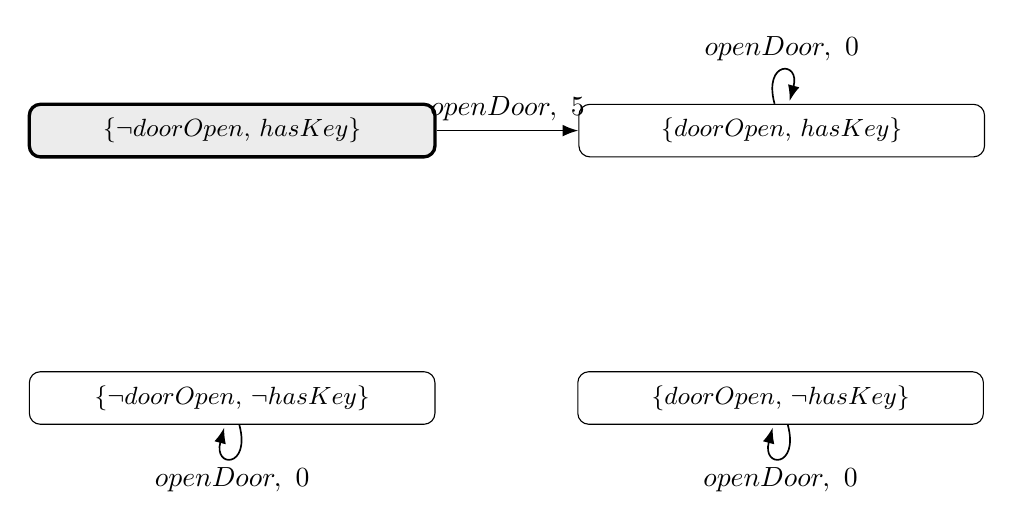
\begin{tikzpicture}[
    >=Latex,
    node distance=2.7cm and 1.8cm,
    state/.style={
        draw,
        rounded corners,
        align=center,
        text width=4.8cm,
        inner sep=5pt,
        font=\small
    },
    trans/.style={->, semithick}
]
\node[state, very thick, fill=gray!15] (s0) {$\{\neg doorOpen,\, hasKey\}$};
\node[state, right=of s0] (s1) {$\{doorOpen,\, hasKey\}$};
\node[state, below=of s0] (s2) {$\{\neg doorOpen,\, \neg hasKey\}$};
\node[state, right=of s2] (s3) {$\{doorOpen,\, \neg hasKey\}$};

\draw[trans] (s0) -- node[above] {$openDoor,\ 5$} (s1);
\draw[trans] (s1) edge[loop above] node {$openDoor,\ 0$} ();
\draw[trans] (s2) edge[loop below] node {$openDoor,\ 0$} ();
\draw[trans] (s3) edge[loop below] node {$openDoor,\ 0$} ();
\end{tikzpicture}
}
\caption{State-transition graph for Example 1. The initial state \(\sigma_0\) is highlighted.}
\end{figure}

\subsubsection*{Program}
\begin{centeredleftblock}[0.45\textwidth]
\(
P = (openDoor)
\)
\end{centeredleftblock}

\subsubsection*{Execution}

\begin{centeredleftblock}[0.9\textwidth]
\noindent
\begin{minipage}[t]{0.64\linewidth}
\begin{statementblock}
\text{initial state: } \sigma_0 = \{\neg doorOpen, hasKey\} \\
\Psi(openDoor, \sigma_0) = \sigma_1 \\
\Psi^\star((openDoor), \sigma_0) = \sigma_1 = \{doorOpen, hasKey\}
\end{statementblock}
\end{minipage}
\hfill
\begin{minipage}[t]{0.28\linewidth}
\begin{statementblock}
Cost(openDoor, \sigma_0) = 5 \\
Cost^\star(P) = 5
\end{statementblock}
\end{minipage}
\end{centeredleftblock}


\subsubsection{Query Results}

\paragraph{Q1: Goal Satisfaction}
\[
\{doorOpen\} ~\text{after}~ P
\]
is true.

\paragraph{Q2: Executability with Cost}
\[
P ~\text{executable with cost}~ 5
\]
is true.

\paragraph{Q3: Executability with exact Cost}
\[
P ~\text{executable with exact cost}~ 5
\]
is true.

\subsection*{Example 2}
This example shows three different reasons why the cost of an action may be
\(0\): because no cost statement is given, because the action has an empty
effect, and because both conditions hold at the same time.

\scenarioheader
An agent stands in front of a closed door and does not have the key. The key
lies nearby. Taking the key makes the agent have the key. Opening the door
makes the door open if the agent has the key. Opening the door costs 5.
\repheader
\begin{centeredleftblock}[0.62\textwidth]
\begin{statementblock}
\text{initially}~ \neg doorOpen \\
\text{initially}~ \neg hasKey \\
takeKey ~\text{causes}~ hasKey \\
openDoor ~\text{causes}~ doorOpen ~\text{if}~ hasKey \\
openDoor ~\text{costs}~ 5
\end{statementblock}
\end{centeredleftblock}


\exampleblocktitle{Set of all states}
\[
\states = \{\sigma_0, \sigma_1, \sigma_2, \sigma_3\},\text{ where: }
\]
\noindent
\begin{minipage}[t]{0.47\textwidth}
\begin{statementblock}
\sigma_0 = \{\neg doorOpen, \neg hasKey\} \\
\sigma_1 = \{\neg doorOpen, hasKey\}
\end{statementblock}
\end{minipage}
\hfill
\begin{minipage}[t]{0.47\textwidth}
\begin{statementblock}
\sigma_2 = \{doorOpen, \neg hasKey\} \\
\sigma_3 = \{doorOpen, hasKey\}
\end{statementblock}
\end{minipage}

\exampleblocktitle{Transition function}
\noindent
\begin{minipage}[t]{0.47\textwidth}
\begin{statementblock}
\Psi(takeKey, \sigma_0) = \sigma_1 \byrule{(M1), (M2b)} \\
\Psi(takeKey, \sigma_1) = \sigma_1 \byrule{(M1), (M2b)} \\
\Psi(takeKey, \sigma_2) = \sigma_3 \byrule{(M1), (M2b)} \\
\Psi(takeKey, \sigma_3) = \sigma_3 \byrule{(M1), (M2b)}
\end{statementblock}
\end{minipage}
\hfill
\begin{minipage}[t]{0.47\textwidth}
\begin{statementblock}
\Psi(openDoor, \sigma_0) = \sigma_0 \byrule{(M2a), (M2b)} \\
\Psi(openDoor, \sigma_1) = \sigma_3 \byrule{(M1), (M2b)} \\
\Psi(openDoor, \sigma_2) = \sigma_2 \byrule{(M2a), (M2b)} \\
\Psi(openDoor, \sigma_3) = \sigma_3 \byrule{(M1), (M2b)}
\end{statementblock}
\end{minipage}

\exampleblocktitle{Cost function}
\noindent
\begin{minipage}[t]{0.47\textwidth}
\begin{statementblock}
Cost(takeKey, \sigma_0) = 0 \byrule{(C2a)} \\
Cost(takeKey, \sigma_1) = 0 \byrule{(C2a), (C2b)} \\
Cost(takeKey, \sigma_2) = 0 \byrule{(C2a)} \\
Cost(takeKey, \sigma_3) = 0 \byrule{(C2a), (C2b)}
\end{statementblock}
\end{minipage}
\hfill
\begin{minipage}[t]{0.47\textwidth}
\begin{statementblock}
Cost(openDoor, \sigma_0) = 0 \byrule{(C2b)} \\
Cost(openDoor, \sigma_1) = 5 \byrule{(C1)} \\
Cost(openDoor, \sigma_2) = 0 \byrule{(C2b)} \\
Cost(openDoor, \sigma_3) = 0 \byrule{(C2b)}
\end{statementblock}
\end{minipage}

\begin{figure}[H]
\centering
\setlength{\fboxsep}{8pt}
\fbox{%
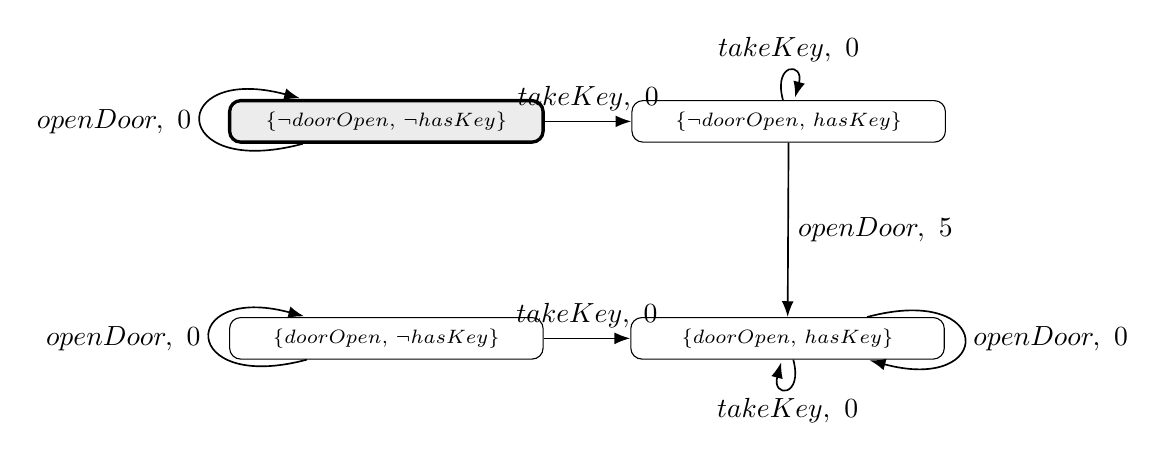
\begin{tikzpicture}[
    >=Latex,
    node distance=2.2cm and 1.1cm,
    state/.style={
        draw,
        rounded corners,
        align=center,
        text width=3.7cm,
        inner sep=4pt,
        font=\scriptsize
    },
    trans/.style={->, semithick}
]
\node[state, very thick, fill=gray!15] (s0) {$\{\neg doorOpen,\, \neg hasKey\}$};
\node[state, right=of s0] (s1) {$\{\neg doorOpen,\, hasKey\}$};
\node[state, below=of s0] (s2) {$\{doorOpen,\, \neg hasKey\}$};
\node[state, right=of s2] (s3) {$\{doorOpen,\, hasKey\}$};

\draw[trans] (s0) -- node[above] {$takeKey,\ 0$} (s1);
\draw[trans] (s2) -- node[above] {$takeKey,\ 0$} (s3);
\draw[trans] (s1) edge[loop above] node {$takeKey,\ 0$} ();
\draw[trans] (s3) edge[loop below] node {$takeKey,\ 0$} ();
\draw[trans] (s0) edge[loop left] node {$openDoor,\ 0$} ();
\draw[trans] (s2) edge[loop left] node {$openDoor,\ 0$} ();
\draw[trans] (s1) -- node[right] {$openDoor,\ 5$} (s3);
\draw[trans] (s3) edge[loop right] node {$openDoor,\ 0$} ();
\end{tikzpicture}
}
\caption{State-transition graph for Example 2.}
\end{figure}

\subsubsection*{Program}
\begin{centeredleftblock}[0.5\textwidth]
\(
P = (takeKey, takeKey, openDoor, openDoor)
\)
\end{centeredleftblock}

\subsubsection*{Execution}
\begin{centeredleftblock}[0.92\textwidth]
\noindent
\begin{minipage}[t]{0.64\linewidth}
\begin{statementblock}
\text{initial state: } \sigma_0 = \{\neg doorOpen, \neg hasKey\} \\
\Psi(takeKey, \sigma_0) = \sigma_1 = \{\neg doorOpen, hasKey\} \\
\Psi(takeKey, \sigma_1) = \sigma_1 = \{\neg doorOpen, hasKey\} \\
\Psi(openDoor, \sigma_1) = \sigma_3 = \{doorOpen, hasKey\} \\
\Psi(openDoor, \sigma_3) = \sigma_3 = \{doorOpen, hasKey\} \\
\Psi^\star(P, \sigma_0) = \sigma_3 = \{doorOpen, hasKey\}
\end{statementblock}
\end{minipage}
\hfill
\begin{minipage}[t]{0.28\linewidth}
\begin{statementblock}
Cost(takeKey, \sigma_0) = 0 \\
Cost(takeKey, \sigma_1) = 0 \\
Cost(openDoor, \sigma_1) = 5 \\
Cost(openDoor, \sigma_3) = 0 \\
Cost^\star(P) = 5
\end{statementblock}
\end{minipage}
\end{centeredleftblock}

\subsubsection*{Final States}
\[
\{\sigma_3\}
\]


\subsubsection*{Query Results}

\paragraph{Q1: Goal Satisfaction}
\[
\{doorOpen, hasKey\} ~\text{after}~ P
\]
is true.

\paragraph{Q2: Executability with Cost}
\[
P ~\text{executable with cost}~ 5
\]
is true.

\paragraph{Q3: Executability with exact Cost}
\[
P ~\text{executable with exact cost}~ 5
\]
is true.

\[
takeKey ~\text{executable with exact cost}~ 0
\]
is true because no cost statement is declared for \(takeKey\), so this is case
\((C2a)\).

\[
takeKey, takeKey ~\text{executable with exact cost}~ 0
\]
is true because the second occurrence of \(takeKey\) has both no declared cost
and an empty effect, so both \((C2a)\) and \((C2b)\) apply.

\[
openDoor, openDoor ~\text{executable with exact cost}~ 5
\]
is true because the first occurrence uses \((C1)\), while the second
occurrence has an empty effect and therefore uses \((C2b)\).

\subsection*{Example 3}
This example shows how a partial description of the initial state leads to
multiple models, different executions of the same program, and different total
costs.

\scenarioheader
An agent stands in front of a closed storage room door. It is unknown whether
the agent already has the key, but a spare key hangs nearby. Taking the key
makes the agent have the key. Opening the door makes the door open if the
agent has the key. Taking the key costs 1. Opening the door costs 5.

\repheader
\begin{centeredleftblock}[0.62\textwidth]
\begin{statementblock}
\text{initially}~ \neg doorOpen \\
takeKey ~\text{causes}~ hasKey \\
takeKey ~\text{costs}~ 1 \\
openDoor ~\text{causes}~ doorOpen ~\text{if}~ hasKey \\
openDoor ~\text{costs}~ 5
\end{statementblock}
\end{centeredleftblock}


\exampleblocktitle{Set of all states}
\[
\states = \{\sigma_0, \sigma_1, \sigma_2, \sigma_3\},\text{ where: }
\]
\noindent
\begin{minipage}[t]{0.47\textwidth}
\begin{statementblock}
\sigma_0 = \{\neg doorOpen, hasKey\} \\
\sigma_1 = \{doorOpen, hasKey\}
\end{statementblock}
\end{minipage}
\hfill
\begin{minipage}[t]{0.47\textwidth}
\begin{statementblock}
\sigma_2 = \{\neg doorOpen, \neg hasKey\} \\
\sigma_3 = \{doorOpen, \neg hasKey\}
\end{statementblock}
\end{minipage}

\exampleblocktitle{Transition function}
\noindent
\begin{minipage}[t]{0.47\textwidth}
\begin{statementblock}
\Psi(takeKey, \sigma_0) = \sigma_0 \byrule{(M1), (M2b)} \\
\Psi(takeKey, \sigma_1) = \sigma_1 \byrule{(M1), (M2b)} \\
\Psi(takeKey, \sigma_2) = \sigma_0 \byrule{(M1), (M2b)} \\
\Psi(takeKey, \sigma_3) = \sigma_1 \byrule{(M1), (M2b)}
\end{statementblock}
\end{minipage}
\hfill
\begin{minipage}[t]{0.47\textwidth}
\begin{statementblock}
\Psi(openDoor, \sigma_0) = \sigma_1 \byrule{(M1), (M2b)} \\
\Psi(openDoor, \sigma_1) = \sigma_1 \byrule{(M1), (M2b)} \\
\Psi(openDoor, \sigma_2) = \sigma_2 \byrule{(M2a), (M2b)} \\
\Psi(openDoor, \sigma_3) = \sigma_3 \byrule{(M2a), (M2b)}
\end{statementblock}
\end{minipage}

\exampleblocktitle{Cost function}
\noindent
\begin{minipage}[t]{0.47\textwidth}
\begin{statementblock}
Cost(takeKey, \sigma_0) = 0 \byrule{(C2b)} \\
Cost(takeKey, \sigma_1) = 0 \byrule{(C2b)} \\
Cost(takeKey, \sigma_2) = 1 \byrule{(C1)} \\
Cost(takeKey, \sigma_3) = 1 \byrule{(C1)}
\end{statementblock}
\end{minipage}
\hfill
\begin{minipage}[t]{0.47\textwidth}
\begin{statementblock}
Cost(openDoor, \sigma_0) = 5 \byrule{(C1)} \\
Cost(openDoor, \sigma_1) = 0 \byrule{(C2b)} \\
Cost(openDoor, \sigma_2) = 0 \byrule{(C2b)} \\
Cost(openDoor, \sigma_3) = 0 \byrule{(C2b)}
\end{statementblock}
\end{minipage}

Due to the partial description of the initial state, we have two models:
\[
S_1 = (\Psi, \sigma_0, Cost), \qquad S_2 = (\Psi, \sigma_2, Cost).
\]

\subsubsection*{Program}
\begin{centeredleftblock}[0.56\textwidth]
\(
P = (openDoor, takeKey, openDoor)
\)
\end{centeredleftblock}

\subsubsection*{Model 1}
For model \(S_1\), the initial state is \(\sigma_0 = \{\neg doorOpen, hasKey\}\).
\begin{figure}[H]
\centering
\setlength{\fboxsep}{8pt}
\fbox{%
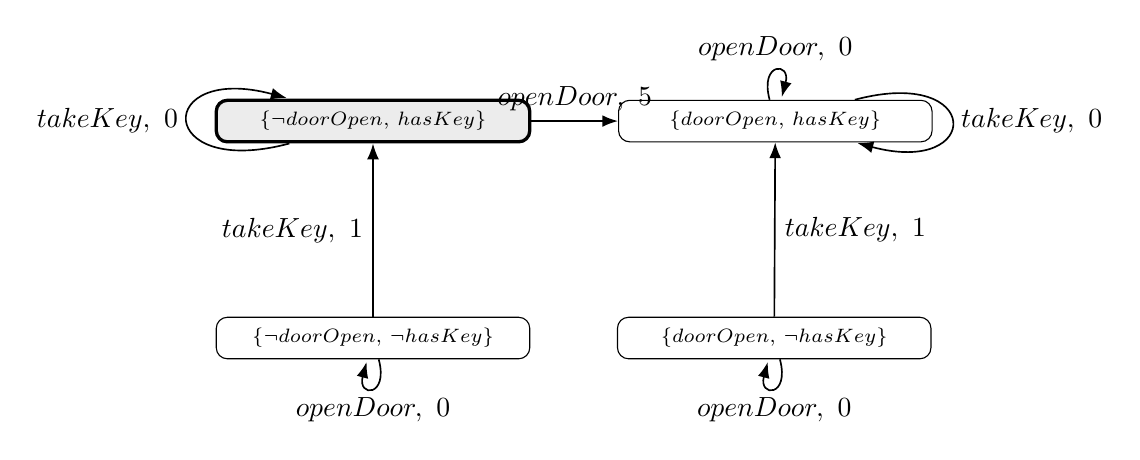
\begin{tikzpicture}[
    >=Latex,
    node distance=2.2cm and 1.1cm,
    state/.style={
        draw,
        rounded corners,
        align=center,
        text width=3.7cm,
        inner sep=4pt,
        font=\scriptsize
    },
    trans/.style={->, semithick}
]
\node[state, very thick, fill=gray!15] (s0) {$\{\neg doorOpen,\, hasKey\}$};
\node[state, right=of s0] (s1) {$\{doorOpen,\, hasKey\}$};
\node[state, below=of s0] (s2) {$\{\neg doorOpen,\, \neg hasKey\}$};
\node[state, right=of s2] (s3) {$\{doorOpen,\, \neg hasKey\}$};

\draw[trans] (s0) -- node[above] {$openDoor,\ 5$} (s1);
\draw[trans] (s1) edge[loop above] node {$openDoor,\ 0$} ();
\draw[trans] (s2) edge[loop below] node {$openDoor,\ 0$} ();
\draw[trans] (s3) edge[loop below] node {$openDoor,\ 0$} ();
\draw[trans] (s0) edge[loop left] node {$takeKey,\ 0$} ();
\draw[trans] (s1) edge[loop right] node {$takeKey,\ 0$} ();
\draw[trans] (s2) -- node[left] {$takeKey,\ 1$} (s0);
\draw[trans] (s3) -- node[right] {$takeKey,\ 1$} (s1);
\end{tikzpicture}
}
\caption{State-transition graph for Example 3 in Model 1.}
\end{figure}

\subsubsection*{Execution in Model 1}
\begin{centeredleftblock}[0.9\textwidth]
\noindent
\begin{minipage}[t]{0.64\linewidth}
\begin{statementblock}
\text{initial state: } \sigma_0 = \{\neg doorOpen, hasKey\} \\
\Psi(openDoor, \sigma_0) = \sigma_1 = \{doorOpen, hasKey\} \\
\Psi(takeKey, \sigma_1) = \sigma_1 = \{doorOpen, hasKey\} \\
\Psi(openDoor, \sigma_1) = \sigma_1 = \{doorOpen, hasKey\} \\
\Psi^\star(P, \sigma_0) = \sigma_1 = \{doorOpen, hasKey\}
\end{statementblock}
\end{minipage}
\hfill
\begin{minipage}[t]{0.28\linewidth}
\begin{statementblock}
Cost(openDoor, \sigma_0) = 5 \\
Cost(takeKey, \sigma_1) = 0 \\
Cost(openDoor, \sigma_1) = 0 \\
Cost^\star(P) = 5
\end{statementblock}
\end{minipage}
\end{centeredleftblock}

\subsubsection*{Model 2}
For model \(S_2\), the initial state is \(\sigma_2 = \{\neg doorOpen, \neg hasKey\}\).

\begin{figure}[H]
\centering
\setlength{\fboxsep}{8pt}
\fbox{%
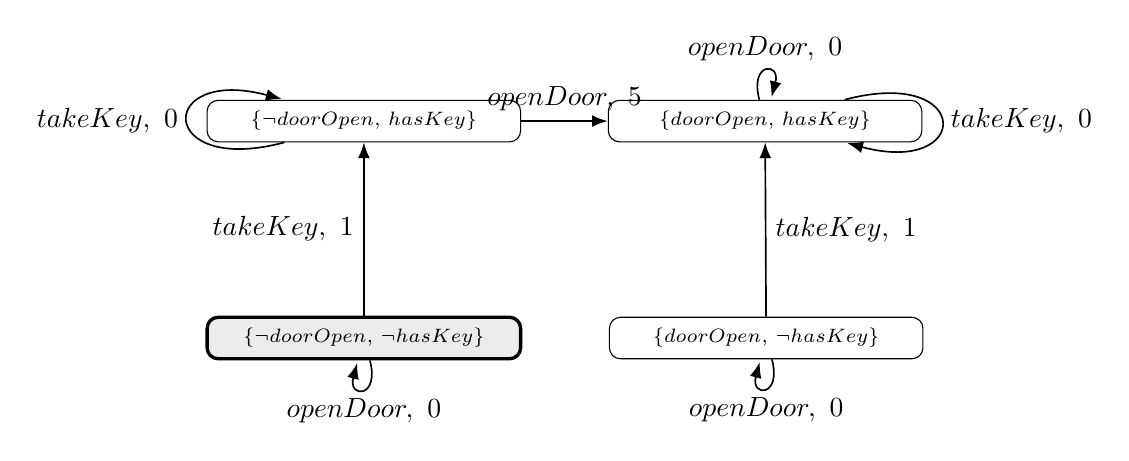
\begin{tikzpicture}[
    >=Latex,
    node distance=2.2cm and 1.1cm,
    state/.style={
        draw,
        rounded corners,
        align=center,
        text width=3.7cm,
        inner sep=4pt,
        font=\scriptsize
    },
    trans/.style={->, semithick}
]
\node[state] (s0) {$\{\neg doorOpen,\, hasKey\}$};
\node[state, right=of s0] (s1) {$\{doorOpen,\, hasKey\}$};
\node[state, very thick, fill=gray!15, below=of s0] (s2) {$\{\neg doorOpen,\, \neg hasKey\}$};
\node[state, right=of s2] (s3) {$\{doorOpen,\, \neg hasKey\}$};

\draw[trans] (s0) -- node[above] {$openDoor,\ 5$} (s1);
\draw[trans] (s1) edge[loop above] node {$openDoor,\ 0$} ();
\draw[trans] (s2) edge[loop below] node {$openDoor,\ 0$} ();
\draw[trans] (s3) edge[loop below] node {$openDoor,\ 0$} ();
\draw[trans] (s0) edge[loop left] node {$takeKey,\ 0$} ();
\draw[trans] (s1) edge[loop right] node {$takeKey,\ 0$} ();
\draw[trans] (s2) -- node[left] {$takeKey,\ 1$} (s0);
\draw[trans] (s3) -- node[right] {$takeKey,\ 1$} (s1);
\end{tikzpicture}
}
\caption{State-transition graph for Example 3 in Model 2.}
\end{figure}

\subsubsection*{Execution in Model 2}
\begin{centeredleftblock}[0.9\textwidth]
\noindent
\begin{minipage}[t]{0.64\linewidth}
\begin{statementblock}
\text{initial state: } \sigma_2 = \{\neg doorOpen, \neg hasKey\} \\
\Psi(openDoor, \sigma_2) = \sigma_2 = \{\neg doorOpen, \neg hasKey\} \\
\Psi(takeKey, \sigma_2) = \sigma_0 = \{\neg doorOpen, hasKey\} \\
\Psi(openDoor, \sigma_0) = \sigma_1 = \{doorOpen, hasKey\} \\
\Psi^\star(P, \sigma_2) = \sigma_1 = \{doorOpen, hasKey\}
\end{statementblock}
\end{minipage}
\hfill
\begin{minipage}[t]{0.28\linewidth}
\begin{statementblock}
Cost(openDoor, \sigma_2) = 0 \\
Cost(takeKey, \sigma_2) = 1 \\
Cost(openDoor, \sigma_0) = 5 \\
Cost^\star(P) = 6
\end{statementblock}
\end{minipage}
\end{centeredleftblock}

\subsubsection*{Query Results}

\paragraph{Q1: Goal Satisfaction}
\[
\{doorOpen\} ~\text{after}~ P
\]
is true because $doorOpen$ holds in the final state of every model.

\paragraph{Q2: Executability with Cost}
\[
P ~\text{executable with cost}~ 6
\]
is true since in every execution:
\[
Cost^\star(P) \leq 6
\]

\paragraph{Q3: Executability with exact Cost}
\[
P ~\text{executable with exact cost}~ 6
\]
is false because \(Cost^\star(P) = 5\) in model \(S_1\), while
\(Cost^\star(P) = 6\) in model \(S_2\).


\subsection*{Example 4}
This example shows how a value statement can impose the initial state.

\scenarioheader
An agent stands in front of a closed door. It is unknown whether the agent
already has the key, but a spare key hangs nearby. Taking the key makes the
agent have the key. Opening the door makes the door open if the agent has the
key. Taking the key costs 1. Opening the door costs 5. After 
opening the door, the door is open.


\repheader
\begin{centeredleftblock}[0.62\textwidth]
\begin{statementblock}
\text{initially}~ \neg doorOpen \\
doorOpen ~\text{after}~ openDoor \\
takeKey ~\text{causes}~ hasKey \\
takeKey ~\text{costs}~ 1 \\
openDoor ~\text{causes}~ doorOpen ~\text{if}~ hasKey \\
openDoor ~\text{costs}~ 5
\end{statementblock}
\end{centeredleftblock}

\subsubsection*{Imposition of the Initial State}
The partial description of the initial state gives two candidate complete
initial states:
\[
\sigma_0 = \{\neg doorOpen, hasKey\}
\]
\[
\sigma_2 = \{\neg doorOpen, \neg hasKey\}
\]
However, the value statement
\[
doorOpen ~\text{after}~ openDoor
\]
eliminates \(\sigma_2\), because
\[
\Psi^\star((openDoor), \sigma_2) = \sigma_0 = \{\neg doorOpen, hasKey\},
\]
and \(doorOpen\) does not hold in the resulting state.

Therefore, the only model of the domain is
\[
S = (\Psi, \sigma_0, Cost).
\]

\exampleblocktitle{Set of all states}
\[
\states = \{\sigma_0, \sigma_1, \sigma_2, \sigma_3\},\text{ where: }
\]
\noindent
\begin{minipage}[t]{0.47\textwidth}
\begin{statementblock}
\sigma_0 = \{\neg doorOpen, hasKey\} \\
\sigma_1 = \{doorOpen, hasKey\}
\end{statementblock}
\end{minipage}
\hfill
\begin{minipage}[t]{0.47\textwidth}
\begin{statementblock}
\sigma_2 = \{\neg doorOpen, \neg hasKey\} \\
\sigma_3 = \{doorOpen, \neg hasKey\}
\end{statementblock}
\end{minipage}

\exampleblocktitle{Transition function}
\noindent
\begin{minipage}[t]{0.47\textwidth}
\begin{statementblock}
\Psi(takeKey, \sigma_0) = \sigma_0 \byrule{(M1), (M2b)} \\
\Psi(takeKey, \sigma_1) = \sigma_1 \byrule{(M1), (M2b)} \\
\Psi(takeKey, \sigma_2) = \sigma_0 \byrule{(M1), (M2b)} \\
\Psi(takeKey, \sigma_3) = \sigma_1 \byrule{(M1), (M2b)}
\end{statementblock}
\end{minipage}
\hfill
\begin{minipage}[t]{0.47\textwidth}
\begin{statementblock}
\Psi(openDoor, \sigma_0) = \sigma_1 \byrule{(M1), (M2b)} \\
\Psi(openDoor, \sigma_1) = \sigma_1 \byrule{(M1), (M2b)} \\
\Psi(openDoor, \sigma_2) = \sigma_2 \byrule{(M2a), (M2b)} \\
\Psi(openDoor, \sigma_3) = \sigma_3 \byrule{(M2a), (M2b)}
\end{statementblock}
\end{minipage}

\exampleblocktitle{Cost function}
\noindent
\begin{minipage}[t]{0.47\textwidth}
\begin{statementblock}
Cost(takeKey, \sigma_0) = 0 \byrule{(C2b)} \\
Cost(takeKey, \sigma_1) = 0 \byrule{(C2b)} \\
Cost(takeKey, \sigma_2) = 1 \byrule{(C1)} \\
Cost(takeKey, \sigma_3) = 1 \byrule{(C1)}
\end{statementblock}
\end{minipage}
\hfill
\begin{minipage}[t]{0.47\textwidth}
\begin{statementblock}
Cost(openDoor, \sigma_0) = 5 \byrule{(C1)} \\
Cost(openDoor, \sigma_1) = 0 \byrule{(C2b)} \\
Cost(openDoor, \sigma_2) = 0 \byrule{(C2b)} \\
Cost(openDoor, \sigma_3) = 0 \byrule{(C2b)}
\end{statementblock}
\end{minipage}

\begin{figure}[H]
\centering
\setlength{\fboxsep}{8pt}
\fbox{%
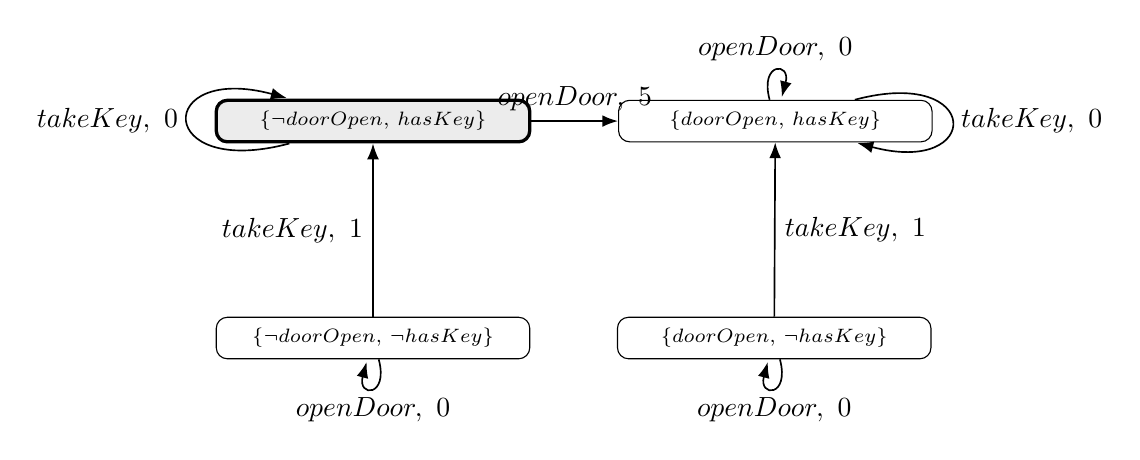
\begin{tikzpicture}[
    >=Latex,
    node distance=2.2cm and 1.1cm,
    state/.style={
        draw,
        rounded corners,
        align=center,
        text width=3.7cm,
        inner sep=4pt,
        font=\scriptsize
    },
    trans/.style={->, semithick}
]
\node[state, very thick, fill=gray!15] (s0) {$\{\neg doorOpen,\, hasKey\}$};
\node[state, right=of s0] (s1) {$\{doorOpen,\, hasKey\}$};
\node[state, below=of s0] (s2) {$\{\neg doorOpen,\, \neg hasKey\}$};
\node[state, right=of s2] (s3) {$\{doorOpen,\, \neg hasKey\}$};

\draw[trans] (s0) -- node[above] {$openDoor,\ 5$} (s1);
\draw[trans] (s1) edge[loop above] node {$openDoor,\ 0$} ();
\draw[trans] (s2) edge[loop below] node {$openDoor,\ 0$} ();
\draw[trans] (s3) edge[loop below] node {$openDoor,\ 0$} ();
\draw[trans] (s0) edge[loop left] node {$takeKey,\ 0$} ();
\draw[trans] (s1) edge[loop right] node {$takeKey,\ 0$} ();
\draw[trans] (s2) -- node[left] {$takeKey,\ 1$} (s0);
\draw[trans] (s3) -- node[right] {$takeKey,\ 1$} (s1);
\end{tikzpicture}
}
\caption{State-transition graph for Example 4.}
\end{figure}

\subsubsection*{Program}
\begin{centeredleftblock}[0.56\textwidth]
\(
P = (openDoor, takeKey)
\)
\end{centeredleftblock}


\subsubsection*{Execution}
\begin{centeredleftblock}[0.9\textwidth]
\noindent
\begin{minipage}[t]{0.64\linewidth}
\begin{statementblock}
\text{initial state: } \sigma_0 = \{\neg doorOpen, hasKey\} \\
\Psi(openDoor, \sigma_0) = \sigma_1 = \{doorOpen, hasKey\} \\
\Psi(takeKey, \sigma_1) = \sigma_1 = \{doorOpen, hasKey\} \\
\Psi^\star(P, \sigma_0) = \sigma_1 = \{doorOpen, hasKey\}
\end{statementblock}
\end{minipage}
\hfill
\begin{minipage}[t]{0.28\linewidth}
\begin{statementblock}
Cost(openDoor, \sigma_0) = 5 \\
Cost(takeKey, \sigma_1) = 0 \\
Cost^\star(P) = 5
\end{statementblock}
\end{minipage}
\end{centeredleftblock}

\subsubsection*{Query Results}

\paragraph{Q1: Goal Satisfaction}
\[
\{doorOpen\} ~\text{after}~ P
\]
is true.

\paragraph{Q2: Executability with Cost}
\[
P ~\text{executable with cost}~ 5
\]
is true.

\paragraph{Q3: Executability with exact Cost}
\[
P ~\text{executable with exact cost}~ 5
\]
is true.

\subsection*{Example 5}
This final example shows an inconsistent domain.
\scenarioheader
An agent stands in front of a closed door and does not have the key, but a
spare key hangs nearby. Taking the key makes the agent have the key. Opening
the door makes the door open only if the agent has the key. Taking the key
costs 1. Opening the door costs 5. After opening the door, the door is open.

\repheader
\begin{centeredleftblock}[0.62\textwidth]
\begin{statementblock}
\text{initially}~ \neg doorOpen \\
\text{initially}~ \neg hasKey \\
doorOpen ~\text{after}~ openDoor \\
takeKey ~\text{causes}~ hasKey \\
takeKey ~\text{costs}~ 1 \\
openDoor ~\text{causes}~ doorOpen ~\text{if}~ hasKey \\
openDoor ~\text{costs}~ 5
\end{statementblock}
\end{centeredleftblock}
There is no model satisfying all statements, because the initial state is fixed as
\(\{\neg doorOpen, \neg hasKey\}\). When \(openDoor\) is executed in this state,
the agent does not have the key, so the effect statement
\[
openDoor ~\text{causes}~ doorOpen ~\text{if}~ hasKey
\]
is not applicable. Hence, by inertia, \(doorOpen\) remains false after \(openDoor\).
However, the value statement
\[
doorOpen ~\text{after}~ openDoor
\]
requires \(doorOpen\) to be true after this action. These requirements contradict
each other, so no model of the action domain exists.

These constraints are inconsistent, so no model of the action domain exists.



\section{Technical description}
The compiler was implemented in Python as a pipeline with five main stages:
input normalization, parsing, model construction, query evaluation, and result
presentation. The implementation follows the formal semantics of the
\(\mathbb{DS}_{4}\) action language used in this project.

\subsection{Data structures}
The source specification is first normalized by removing comments and optional
trailing dots. Every non-empty line is stored together with its original line
number, which allows the compiler to report precise parsing errors.

The internal representation is built from several small logical structures:
\begin{itemize}
    \item \textbf{Literal} stores a fluent and its polarity, for example
    \(doorOpen\) or \(!doorOpen\).
    \item \textbf{Value statement} stores a literal and a program, representing
    either an initial fact or a statement of the form
    \(f ~\text{after}~ A_1,\ldots,A_n\).
    \item \textbf{Effect statement} stores an action, a resulting literal,
    and a tuple of preconditions.
    \item \textbf{Cost statement} stores an action and its declared cost.
    \item \textbf{Query structures} represent the three supported query types:
    goal queries, bounded-cost queries, and exact-cost queries.
\end{itemize}

At the domain level, statements are grouped into three tuples:
value statements, effect statements, and cost statements.
This makes later validation and evaluation simpler.

\subsection{Representation of states and programs}
The set of fluents and actions is inferred automatically from the domain.
After that, each fluent is assigned an index. A complete state is represented
as a tuple of Boolean values. If the fluent order is
\((doorOpen, hasKey, alarmActive)\), then the state
\((False, True, False)\) corresponds to
\(\{\neg doorOpen, hasKey, \neg alarmActive\}\).

To access values efficiently, the compiler stores a dictionary mapping each
fluent name to its position in the state tuple. Programs are represented as
tuples of action names.

\subsection{Transition and cost tables}
The core semantic structures are:
\begin{itemize}
    \item a \textbf{transition table} indexed by \((action, state)\), returning
    the next state,
    \item a \textbf{cost table} indexed by \((action, state)\), returning the
    cost of the action in that state,
    \item a tuple of valid initial states, interpreted as the set of models of
    the action domain.
\end{itemize}

This representation is efficient because tuples are immutable and can be used
as dictionary keys. As a consequence, program execution becomes a sequence of
dictionary lookups.

\subsection{Parsing algorithm}
The parser works in the following order:
\begin{enumerate}
    \item normalize the text and split it into the \texttt{[domain]} and
    \texttt{[queries]} sections,
    \item parse every domain line as one of the supported statement forms:
    \texttt{initially ...}, \texttt{... causes ... if ...},
    \texttt{... costs ...}, or \texttt{... after ...},
    \item parse every query line as a goal query, a bounded-cost query,
    or an exact-cost query,
    \item infer the complete signature of fluents and actions from the parsed domain.
\end{enumerate}

The language is small and regular, so direct pattern-based parsing is simpler
and more transparent than using a general parser generator.

\subsection{Model construction algorithm}
Let \(n\) be the number of fluents. The compiler first generates all \(2^n\)
possible complete Boolean assignments. Each assignment is treated as a candidate
initial state.

For every action and every state, the next state is computed as follows:
\begin{enumerate}
    \item start from the current state and apply the inertia law,
    \item collect all effect statements relevant to the given action and fluent,
    \item keep only effects whose preconditions are satisfied,
    \item if no effect is applicable, preserve the old value,
    \item if exactly one truth value is enforced, update the fluent,
    \item if both positive and negative effects apply to the same fluent,
    report a contradiction.
\end{enumerate}

After the transition table is built, the cost table is constructed.
If an action has a declared cost and its execution changes the state, that
cost is used; otherwise the cost is \(0\). This directly implements the
empty-effect rule from the formal semantics.

\subsection{Model filtering and query evaluation}
Not every candidate initial state is a valid model. The compiler removes a state if:
\begin{itemize}
    \item it violates an \texttt{initially} statement, or
    \item after executing a program required by a value statement, the resulting
    state does not satisfy the required literal.
\end{itemize}

The remaining states form the model set of the domain.
Queries are then evaluated universally over this set:
\begin{itemize}
    \item a goal query is true only if the goal holds in the final state of every model,
    \item a bounded-cost query is true only if the total cost never exceeds the bound,
    \item an exact-cost query is true only if every model produces exactly the required cost.
\end{itemize}

If no model remains after filtering, the compiler reports an inconsistent domain
and does not print query results.

\subsection{Complexity}
The dominant cost of the algorithm is state-space generation. Since the number of
candidate states is \(2^n\), the implementation is exponential in the number of
fluents. For this reason it is intended mainly for small and medium-sized
educational examples. The advantage of this exhaustive method is that it stays
very close to the formal semantics and is easy to verify.

\section{Testing}
\subsection*{Michał Szewczak}
\subsection*{Example 1: The Vault Room}
Let's consider a scenario involving a vault room protected by wards and physical security layers and a thief that wants to access the vault illegally. He was given a key, but is not sure whether it is the key to the vault he plans to rob, and has no way to check it. Smashing the door is loud and it triggers the alarm and costs physical effort, but it always opens the door. Picking the lock is elegant and quiet, but it requires the key the thief has to be the right one for the lock to work and bypass the vault's wards, otherwise it completely fails.

\subsubsection*{Action Domain Statements}
\[
\text{initially}~ \neg doorUnlocked
\]
\[
\text{initially}~ \neg alarmActive
\]
\[
doorUnlocked ~\text{after}~ pickLock, smashDoor
\]
\[
pickLock ~\text{causes}~ doorUnlocked ~\text{if}~ hasKey
\]
\[
smashDoor ~\text{causes}~ doorUnlocked
\]
\[
smashDoor ~\text{causes}~ alarmActive
\]
\[
pickLock ~\text{costs}~ 2
\]
\[
smashDoor ~\text{costs}~ 8
\]

\subsubsection*{Program}
\[
P = (pickLock, smashDoor)
\]

\subsubsection*{Complete initial states}
Because the status of the fluent $hasKey$ is left unspecified by the initial historical assumptions, we must generate all possible complete initial states:
\[
\sigma_0^1 = \{\neg doorUnlocked, \neg alarmActive, hasKey\}
\]
\[
\sigma_0^2 = \{\neg doorUnlocked, \neg alarmActive, \neg hasKey\}
\]

\parr
However, $\sigma_0^2$ is not consistent with the value statement constraint in the action domain.
Let us evaluate its branch:
\begin{enumerate}
    \item \textbf{Action 1 ($pickLock$):} Since $hasKey$ does not hold in $\sigma_0^2$, the conditional effect does not apply. By the law of inertia, the state remains completely unchanged:
    \[ \Psi(pickLock, \sigma_0^2) \models \neg doorUnlocked \]
    \item \textbf{Action 2 ($smashDoor$):} The execution continues to the final state:
    \[ \Psi^\star((pickLock, smashDoor), \sigma_0^2) \models doorUnlocked \]
\end{enumerate}
But our structural rules dictate that a multi-step value statement $f ~\text{after}~ A_1, \ldots, A_n$ enforces satisfaction at \emph{every} intermediary path step where that action prefix sequence resolves. The constraint $doorUnlocked ~\text{after}~ pickLock, smashDoor$ demands that:
\[ \Psi(pickLock, \sigma_0^2) \models doorUnlocked \]
This yields a direct contradiction with our step 1 transition evaluation. Therefore, the completion $\sigma_0^2$ is invalid and is completely filtered out of the model construction phase.

\subsubsection*{Execution}
Thus, the only valid, consistent initial state structure is:
\[
\sigma_0 = \{\neg doorUnlocked, \neg alarmActive, hasKey\}
\]

\paragraph{Action 1: $pickLock$}
The precondition $hasKey$ holds true, meaning the postcondition triggers successfully:
\[
\sigma_1 = \{doorUnlocked, \neg alarmActive, hasKey\}
\]
Cost calculation: Since $\Psi(pickLock, \sigma_0) \neq \sigma_0$, the full cost statement maps:
\[
Cost(pickLock, \sigma_0) = 2
\]

\paragraph{Action 2: $smashDoor$}
Both effects of the smashing operation execute unconditionally:
\[
\sigma_2 = \{doorUnlocked, alarmActive, hasKey\}
\]
Cost calculation: While $doorUnlocked$ was already true and remains unchanged, the fluent $alarmActive$ transitions from false to true. Because a state transition occurred ($\Psi(smashDoor, \sigma_1) \neq \sigma_1$), the empty effect rule does not apply:
\[
Cost(smashDoor, \sigma_1) = 8
\]

\paragraph{Total Program Cost}
\[
Cost^\star(P) = 2 + 8 = 10
\]

\subsubsection*{Final States}
\[
\{\sigma_2\}
\]

\subsubsection*{Query Results}

\paragraph{Q1: Goal Satisfaction}
\[
\{doorUnlocked, alarmActive\} ~\text{after}~ pickLock, smashDoor
\]
is true because both literals explicitly hold in the singular final state space model $\sigma_2$.

\paragraph{Q2: Executability with Cost}
\[
pickLock, smashDoor ~\text{executable with cost}~ 10
\]
is true since for all valid executions:
\[
Cost^\star(P) \leq 10
\]

\paragraph{Q3: Executability with exact Cost}
\[
pickLock, smashDoor ~\text{executable with exact cost}~ 10
\]
is true because the alternative inconsistent branch was eliminated, ensuring that $Cost^\star(P) = 10$ holds deterministically across all true models of the domain.

\subsubsection*{Print screen}
\begin{figure}[H]
    \centering
    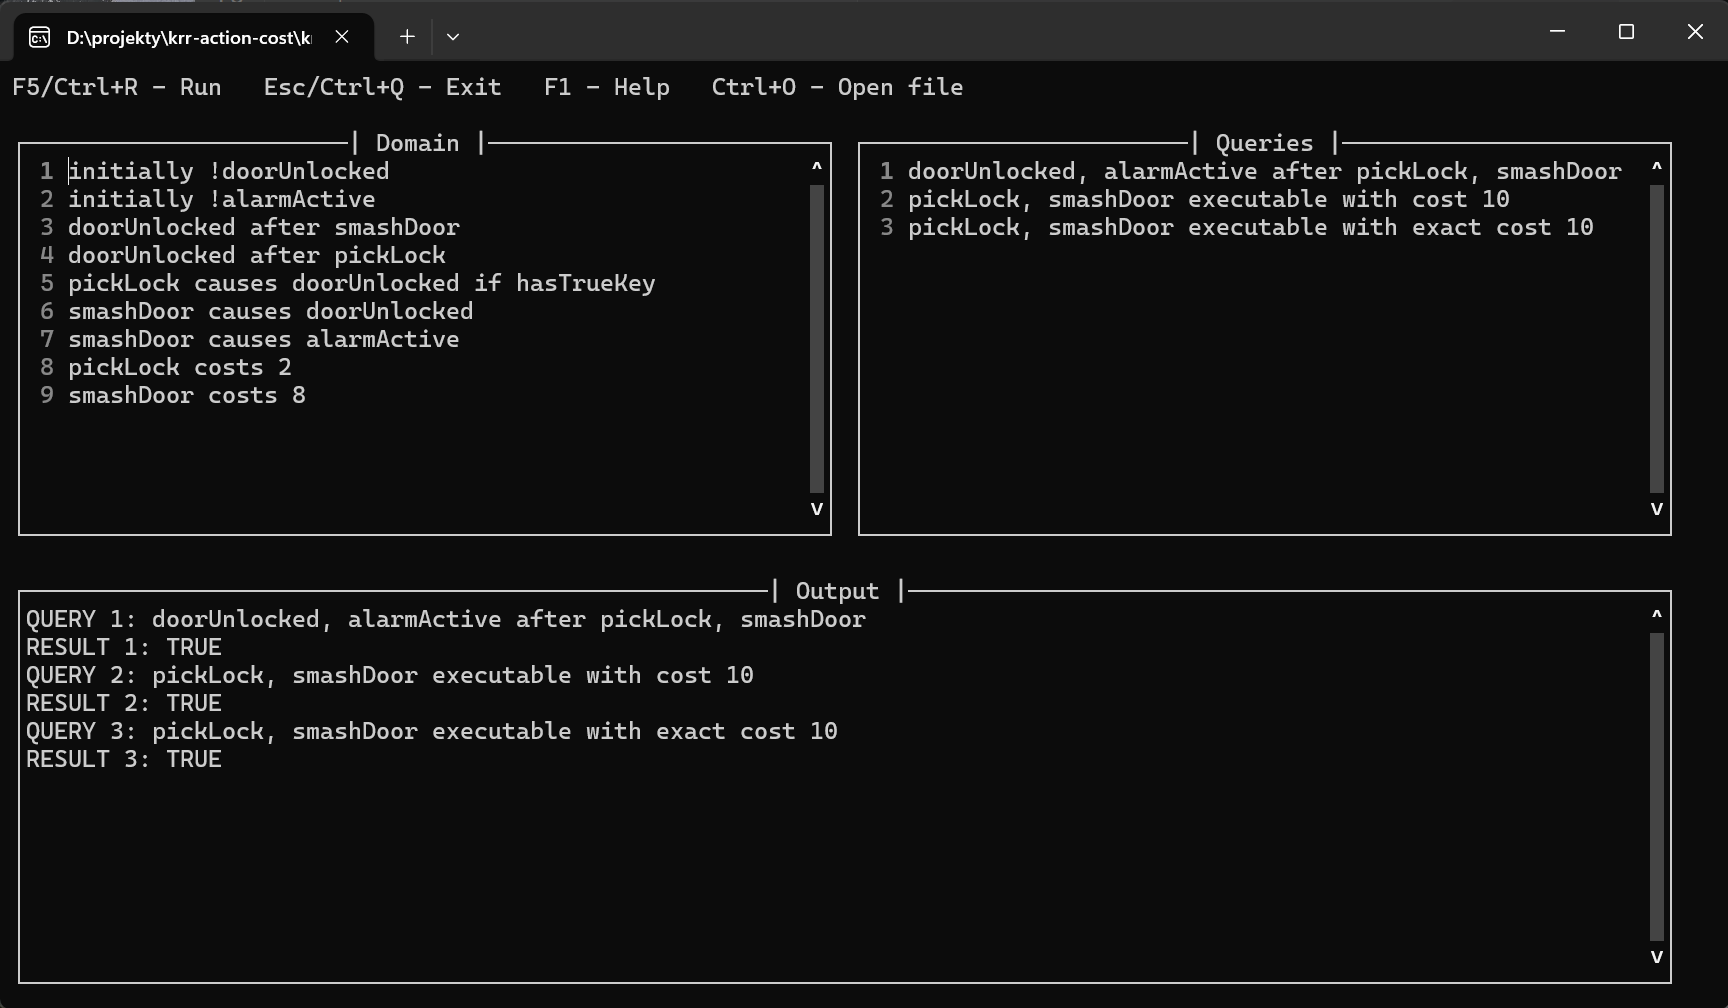
\includegraphics[width=0.8\textwidth]{testing/Michal/example1.png}
    \caption{Michał Szewczak - example 1}
    \label{fig:MS1}
\end{figure}
\subsection{Example 2: The Smart Greenhouse}
Let us consider a scenario in an automated greenhouse where actions may yield empty effects depending on environmental resources.

\subsubsection{Action Domain Statements}
\[
\text{initially}~ soilDry
\]
\[
\text{initially}~ \neg pumpActive
\]
\[
startPump ~\text{causes}~ \neg soilDry ~\text{if}~ \neg waterLow
\]
\[
startPump ~\text{causes}~ pumpActive ~\text{if}~ \neg waterLow
\]
\[
checkReservoir ~\text{causes}~ \neg waterLow
\]
\[
startPump ~\text{costs}~ 5
\]
\[
checkReservoir ~\text{costs}~ 2
\]

\subsubsection{Program}
\[
P = (startPump, checkReservoir)
\]

\subsubsection{Complete initial states}
Since the status of $waterLow$ is omitted from the initial historical properties, the system branches into two valid complete states:
\[
\sigma_0^1 = \{soilDry, \neg pumpActive, \neg waterLow\}
\]
\[
\sigma_0^2 = \{soilDry, \neg pumpActive, waterLow\}
\]

\subsubsection{Execution Path 1 ($\sigma_0^1$)}
\paragraph{Action 1 ($startPump$):} The precondition $\neg waterLow$ holds true. The effects trigger successfully:
\[
\sigma_1^1 = \{\neg soilDry, pumpActive, \neg waterLow\}
\]
Cost calculation: A state change occurred ($\Psi(startPump, \sigma_0^1) \neq \sigma_0^1$), so the full cost is applied:
\[
Cost(startPump, \sigma_0^1) = 5
\]

\paragraph{Action 2 ($checkReservoir$):} The action attempts to ensure water is not low. Because $\neg waterLow$ is already true, the state remains completely identical:
\[
\sigma_2^1 = \{\neg soilDry, pumpActive, \neg waterLow\}
\]
Cost calculation: Since $\Psi(checkReservoir, \sigma_1^1) = \sigma_1^1$, it results in an empty effect, driving the cost to zero:
\[
Cost(checkReservoir, \sigma_1^1) = 0
\]
\[
\text{Total } Cost^\star(P) = 5 + 0 = 5
\]

\subsubsection{Execution Path 2 ($\sigma_0^2$)}
\paragraph{Action 1 ($startPump$):} The precondition $\neg waterLow$ fails. By the law of inertia, no fluents change:
\[
\sigma_1^2 = \{soilDry, \neg pumpActive, waterLow\}
\]
Cost calculation: Because $\Psi(startPump, \sigma_0^2) = \sigma_0^2$, the empty effect rule dictates the cost drops to zero:
\[
Cost(startPump, \sigma_0^2) = 0
\]

\paragraph{Action 2 ($checkReservoir$):} The effect triggers unconditionally, shifting $waterLow$ to false:
\[
\sigma_2^2 = \{soilDry, \neg pumpActive, \neg waterLow\}
\]
Cost calculation: The state successfully changed, forcing the cost assignment:
\[
Cost(checkReservoir, \sigma_1^2) = 2
\]
\[
\text{Total } Cost^\star(P) = 0 + 2 = 2
\]

\subsubsection{Query Results}
\[
P ~\text{executable with cost}~ 4 \quad \text{(False, because } 5 \le 4 \text{ and } 2 \le 4\text{)}
\]
\[
P ~\text{executable with exact cost}~ 4 \quad \text{(False, because program is not even executable with cost 4)}
\]
\subsubsection*{Print screen}
\begin{figure}[H]
    \centering
    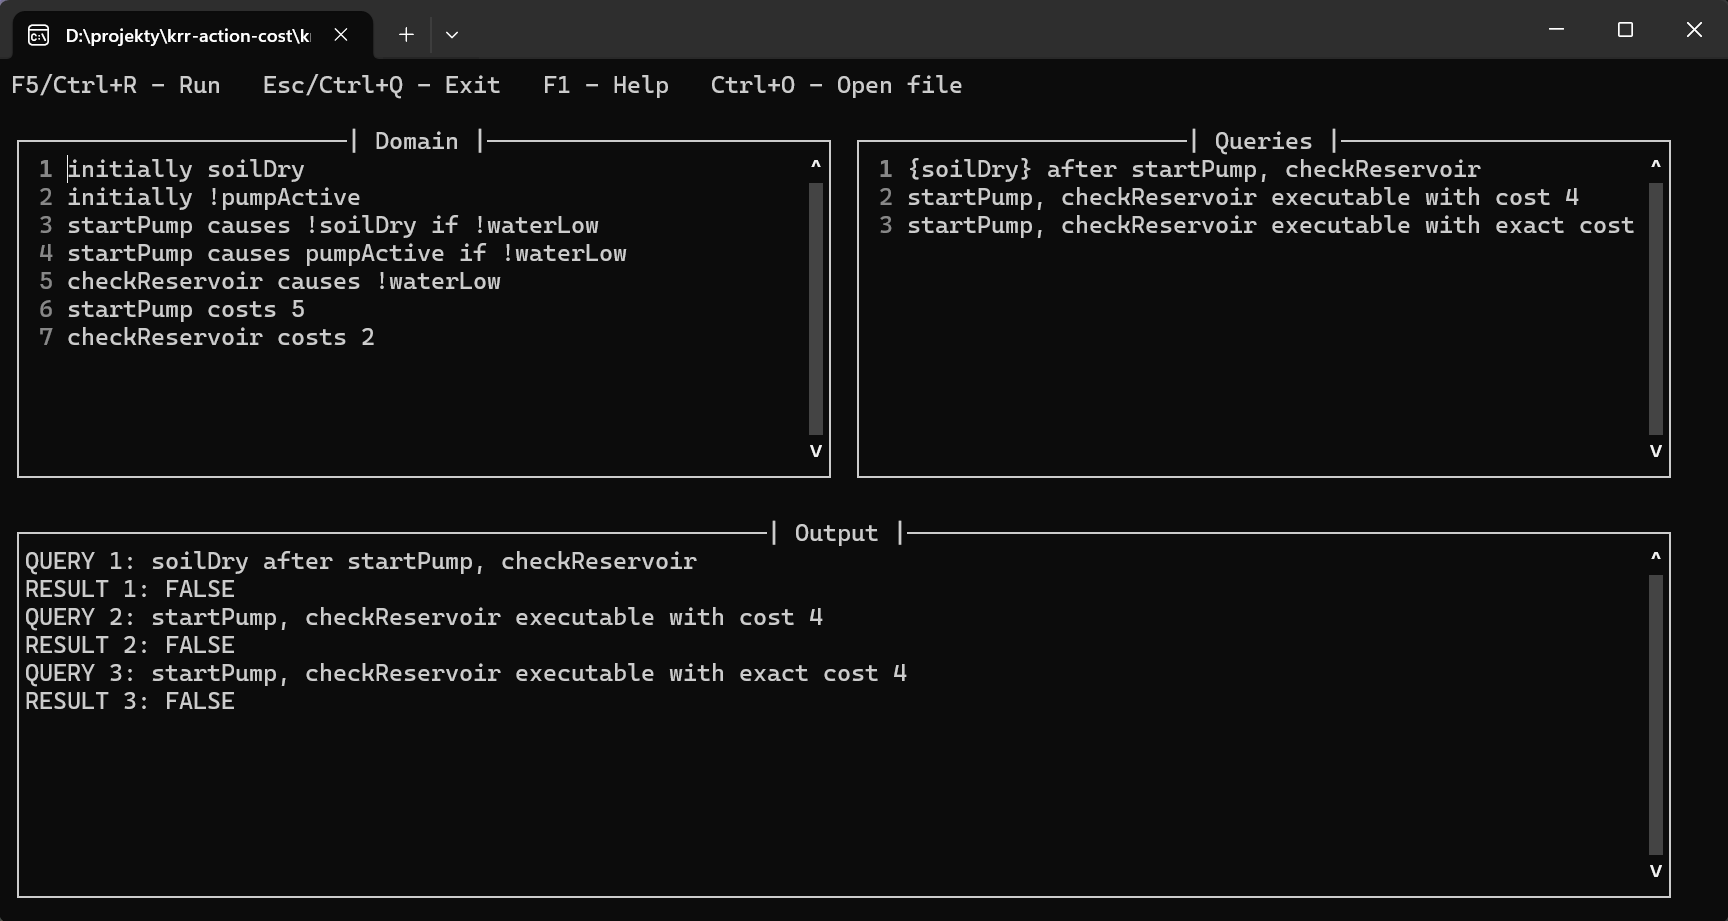
\includegraphics[width=0.8\textwidth]{testing/Michal/example2.png}
    \caption{Michał Szewczak - example 2}
    \label{fig:MS2}
\end{figure}
\subsection{Example 3: The Jammed Door via Single-Action Constraints (Inconsistent Domain)}
This example refines the jammed mechanism scenario by using strictly single-action value statements to enforce a historical observation midway through the plan execution timeline. This formulation exposes the physical impossibility of the system state trajectory, allowing the solver to correctly flag the domain as inconsistent.

\subsubsection{Action Domain Statements}
\[
\text{initially}~ \neg doorOpen
\]
\[
\text{initially}~ \neg doorUnlocked
\]
\[
\text{initially}~ mechanismJammed
\]
\[
doorUnlocked ~\text{after}~ unlockDoor
\]
\[
unlockDoor ~\text{causes}~ doorUnlocked ~\text{if}~ \neg mechanismJammed
\]
\[
forceOpen ~\text{causes}~ doorOpen ~\text{if}~ doorUnlocked
\]
\[
unlockDoor ~\text{costs}~ 3
\]
\[
forceOpen ~\text{costs}~ 5
\]

\subsubsection{Program}
\[
P = (unlockDoor, forceOpen)
\]

\subsubsection{Completions of $\sigma_0$}
The domain completely specifies the values of all system fluents at the origin of time. Hence, the initial configuration generates a single complete state representation:
\[
\sigma_0 = \{\neg doorOpen, \neg doorUnlocked, mechanismJammed\}
\]

\subsubsection{Execution and Consistency Checking}
We evaluate the state transition step-by-step from $\sigma_0$ under the action rules:
\begin{enumerate}
    \item \textbf{Action 1 ($unlockDoor$):} The system attempts to process the transition $\Psi(unlockDoor, \sigma_0)$. The associated effect rule requires that $\neg mechanismJammed$ holds true. However, because $mechanismJammed$ is true in $\sigma_0$, the precondition fails. By the law of inertia, the action produces an empty effect, yielding:
    \[ \sigma_1 = \Psi(unlockDoor, \sigma_0) = \{\neg doorOpen, \neg doorUnlocked, mechanismJammed\} \]
\end{enumerate}

Next, the semantic framework validates the structure against the action language value statement constraints. The domain includes the single-action observation statement:
\[ doorUnlocked ~\text{after}~ unlockDoor \]
By semantic definition, a structure satisfies this statement if and only if the fluent holds in the state immediately following the action's execution:
\[ \Psi(unlockDoor, \sigma_0) \models doorUnlocked \]



However, the transition rules evaluated via inertia explicitly proved that $\sigma_1 \models \neg doorUnlocked$. Because a valid state assignment cannot simultaneously contain a fluent and its logical negation, no transition function can reconcile the observation constraint with the environmental physics.

Therefore, no valid structure exists for this setup, and the system correctly terminates during compilation with the message:
\[ \text{\textbf{The domain is inconsistent.}} \]

\subsubsection{Query Results}
Because no model can be constructed to satisfy the underlying constraints of the dynamic domain, all downstream query validations are structurally precluded from running. The query state evaluations are formally defined as \textbf{undefined}.
\subsubsection*{Print screen}
\begin{figure}[H]
    \centering
    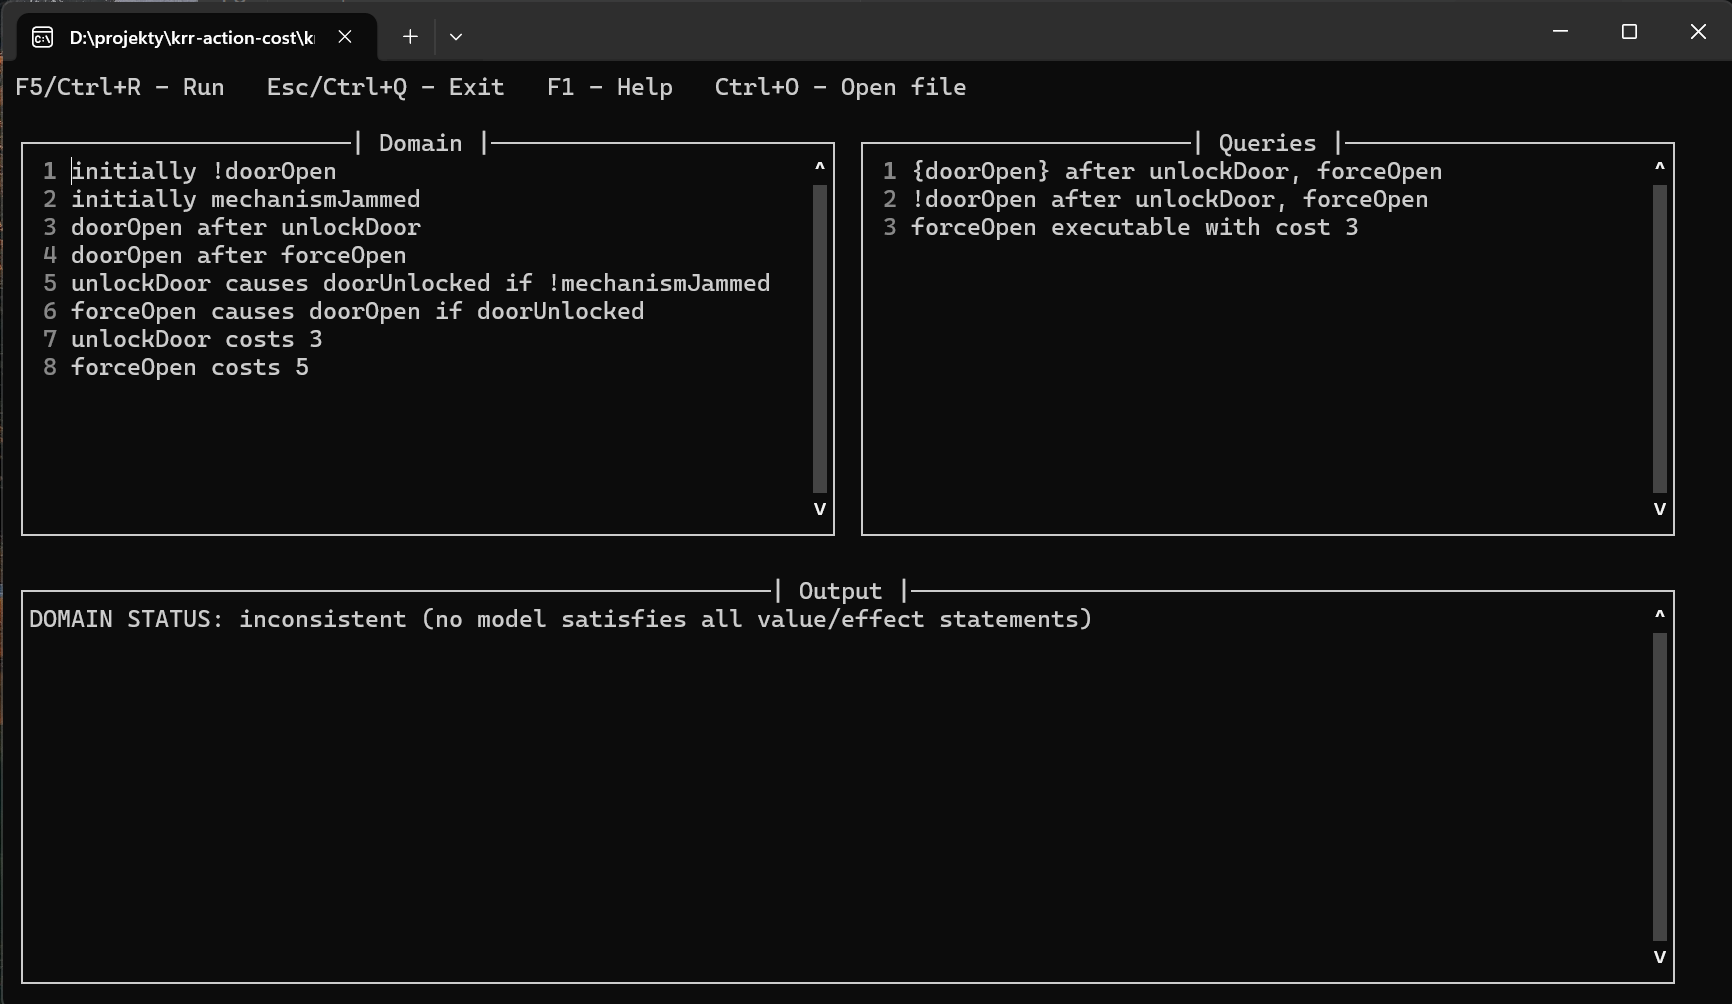
\includegraphics[width=0.8\textwidth]{testing/Michal/example3.png}
    \caption{Michał Szewczak - example 3}
    \label{fig:MS3}
\end{figure}
\subsection{Example 4: The Space Station Airlock (Timeline Convergence)}
An auxiliary airlock chamber is prepared for an emergency spacewalk while flickering hull sensors leave the active status of an external solar storm completely unknown. A manual three-step safety protocol—consisting of chamber depressurization, manual seal unlatching, and hydraulic door release—is executed by an astronaut. Potential variations in external electromagnetic resistance are entirely masked by a heavy hydraulic override system, allowing a completely predictable suit battery drain to be maintained across both possible environmental conditions. This scenario demonstrates a system operating across 4 fluents, 3 actions, and a 3-step execution program. It highlights how an unstated environmental hazard splits the history of the system into branching paths of varying operational costs, which subsequently converge back into a singular, unified final state.

\subsubsection{Action Domain Statements}
\[
\text{initially}~ \neg doorOpen
\]
\[
\text{initially}~ chamberPressurized
\]
\[
\text{initially}~ \neg sealUnlocked
\]
\[
\neg chamberPressurized ~\text{after}~ depressurize
\]
\[
sealUnlocked ~\text{after}~ depressurize, unlatchSeal
\]
\[
depressurize ~\text{causes}~ \neg chamberPressurized
\]
\[
unlatchSeal ~\text{causes}~ sealUnlocked ~\text{if}~ \neg chamberPressurized
\]
\[
openAirlock ~\text{causes}~ doorOpen ~\text{if}~ sealUnlocked
\]
\[
depressurize ~\text{costs}~ 6
\]
\[
unlatchSeal ~\text{costs}~ 2
\]
\[
openAirlock ~\text{costs}~ 5
\]

\subsubsection{Program}
\[
P = (depressurize, unlatchSeal, openAirlock)
\]

\subsubsection{Completions of $\sigma_0$}
The fluent $stormActive$ is omitted from our initial state parameters, branching our framework into two valid, complete initial states:
\[
\sigma_0^1 = \{\neg doorOpen, chamberPressurized, \neg sealUnlocked, \neg stormActive\}
\]
\[
\sigma_0^2 = \{\neg doorOpen, chamberPressurized, \neg sealUnlocked, stormActive\}
\]

\parr
We validate these completions against our single-action historical checkpoints:
\begin{enumerate}
    \item $s_1 = \neg chamberPressurized ~\text{after}~ depressurize$: For both states, running $depressurize$ successfully flips $chamberPressurized \rightarrow \neg chamberPressurized$, satisfying the literal.
    \item $s_2 = sealUnlocked ~\text{after}~ depressurize, unlatchSeal$: Because the first step successfully vented the chamber, the subsequent step $unlatchSeal$ finds its precondition ($\neg chamberPressurized$) satisfied. It flips $\neg sealUnlocked \rightarrow sealUnlocked$ in both timelines.
\end{enumerate}
Both initial state completions are entirely consistent with the tracking observations, meaning both branches survive.

\subsubsection{Execution Paths and Convergence}



\paragraph{Path 1 (No Storm Hazard: $\sigma_0^1$)}
\begin{enumerate}
    \item \textbf{Action 1 ($depressurize$):} The chamber vents. The state changes ($\sigma_1^1 \neq \sigma_0^1$), applying the full power usage:
    \[ \sigma_1^1 = \{\neg doorOpen, \neg chamberPressurized, \neg sealUnlocked, \neg stormActive\} \quad \rightarrow \quad Cost = 6 \]

    \item \textbf{Action 2 ($unlatchSeal$):} Precondition $\neg chamberPressurized$ is true. The seal releases ($\sigma_2^1 \neq \sigma_1^1$):
    \[ \sigma_2^1 = \{\neg doorOpen, \neg chamberPressurized, sealUnlocked, \neg stormActive\} \quad \rightarrow \quad Cost = 2 \]

    \item \textbf{Action 3 ($openAirlock$):} Precondition $sealUnlocked$ is true. The heavy door swings open ($\sigma_3^1 \neq \sigma_2^1$). Since no storm resistance is active, it incurs baseline cost:
    \[ \sigma_3^1 = \{doorOpen, \neg chamberPressurized, sealUnlocked, \neg stormActive\} \quad \rightarrow \quad Cost = 5 \]
\end{enumerate}
\[ \text{Total Path 1 Cost: } Cost^\star(P) = 6 + 2 + 5 = 13 \]

\paragraph{Path 2 (Active Storm Hazard: $\sigma_0^2$)}
\begin{enumerate}
    \item \textbf{Action 1 ($depressurize$):} The chamber vents successfully ($\sigma_1^2 \neq \sigma_0^2$):
    \[ \sigma_1^2 = \{\neg doorOpen, \neg chamberPressurized, \neg sealUnlocked, stormActive\} \quad \rightarrow \quad Cost = 6 \]

    \item \textbf{Action 2 ($unlatchSeal$):} Precondition is true. The seal releases ($\sigma_2^2 \neq \sigma_1^2$):
    \[ \sigma_2^2 = \{\neg doorOpen, \neg chamberPressurized, sealUnlocked, stormActive\} \quad \rightarrow \quad Cost = 2 \]

    \item \textbf{Action 3 ($openAirlock$):} Precondition is true. The outer door opens ($\sigma_3^2 \neq \sigma_2^2$). However, because $stormActive$ is true, the door motor experiences physical counter-force resistance, boosting the execution cost:
    \[ \sigma_3^2 = \{doorOpen, \neg chamberPressurized, sealUnlocked, stormActive\} \quad \rightarrow \quad Cost = 5 \]
\end{enumerate}
\[ \text{Total Path 2 Cost: } Cost^\star(P) = 6 + 2 + 5 = 13 \]

\subsubsection{Final States}
Because the program actions only manipulated mechanical door elements and never interacted with or altered the outer space environment, the fluent $stormActive$ uniquely retains its original divergent values via inertia:
\[
\sigma_3^1 = \{doorOpen, \neg chamberPressurized, sealUnlocked, \neg stormActive\}
\]
\[
\sigma_3^2 = \{doorOpen, \neg chamberPressurized, sealUnlocked, stormActive\}
\]

\subsubsection{Query Results}

\paragraph{Q1: Goal Satisfaction}
\[
\{doorOpen, \neg chamberPressurized, sealUnlocked\} ~\text{after}~ depressurize, unlatchSeal, openAirlock
\]
is \textbf{true} because all three specified goal literals are perfectly satisfied across both final states ($\sigma_3^1$ and $\sigma_3^2$), making the unstated status of the storm irrelevant to final task success.

\paragraph{Q2: Executability with Cost}
\[
depressurize, unlatchSeal, openAirlock ~\text{executable with cost}~ 13
\]
is \textbf{true} since the total cumulative cost across both independent timelines satisfies $13 \le 13$.

\paragraph{Q3: Executability with exact Cost}
\[
depressurize, unlatchSeal, openAirlock ~\text{executable with exact cost}~ 13
\]
is \textbf{true}. Even though the environmental context differed between the branches, their resulting path costs calculated identically, establishing a guaranteed exact cost profile of 13 for the program.
\subsubsection*{Print screen}
\begin{figure}[H]
    \centering
    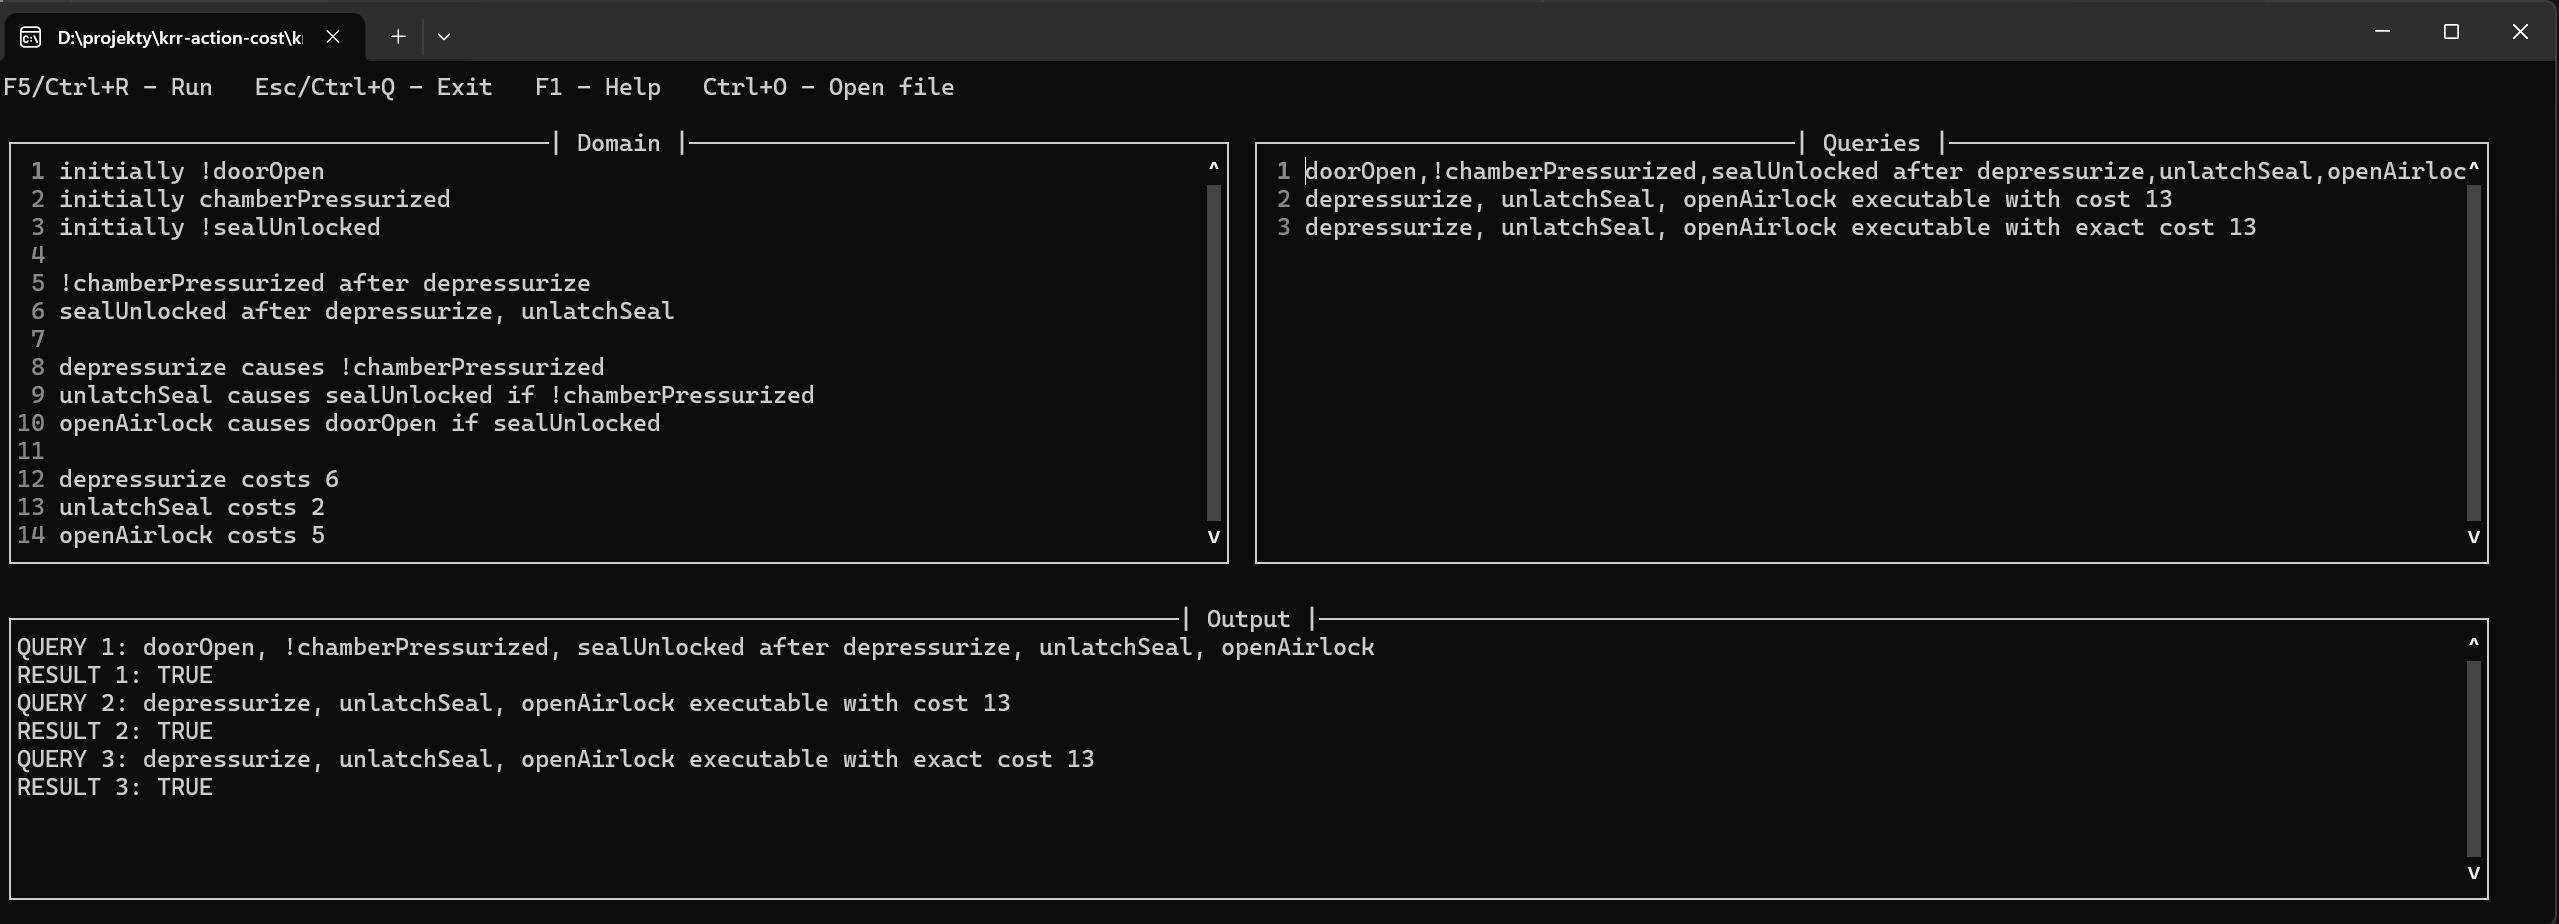
\includegraphics[width=0.8\textwidth]{testing/Michal/example4.png}
    \caption{Michał Szewczak - example 4}
    \label{fig:MS4}
\end{figure}
\subsection*{Jakub Seliga}
\subsection*{Example 1: The Light Switch}
Let's consider a scenario with a light controlled by a switch that can be flipped off and back on, and which can also be permanently locked. Flipping the switch only works while the switch is unlocked; once locked, any further flip has no effect at all.
\subsubsection*{Action Domain Statements}
\[
\text{initially}~ lightOn
\]
\[
\text{initially}~ \neg switchLocked
\]
\[
flipOff ~\text{causes}~ \neg lightOn ~\text{if}~ \neg switchLocked
\]
\[
flipOn ~\text{causes}~ lightOn ~\text{if}~ \neg switchLocked
\]
\[
lockSwitch ~\text{causes}~ switchLocked
\]
\[
flipOff ~\text{costs}~ 3
\]
\[
flipOn ~\text{costs}~ 4
\]
\[
lockSwitch ~\text{costs}~ 1
\]
\subsubsection*{Complete initial states}
Both fluents are fixed by the initial statements, so the initial state is complete and the model is unique:
\[
\sigma_0 = \{lightOn, \neg switchLocked\}
\]
\subsubsection*{Execution}
\paragraph{Program $(flipOff, flipOn)$}
The precondition $\neg switchLocked$ holds, so $flipOff$ turns the light off:
\[
\sigma_1 = \{\neg lightOn, \neg switchLocked\}
\]
\[
Cost(flipOff, \sigma_0) = 3
\]
The precondition still holds, so $flipOn$ turns the light back on:
\[
\sigma_2 = \{lightOn, \neg switchLocked\}
\]
\[
Cost(flipOn, \sigma_1) = 4
\]
\[
Cost^\star(P) = 3 + 4 = 7
\]
\paragraph{Program $(flipOff, flipOff)$}
The first $flipOff$ costs 3 as above. The second $flipOff$ finds $lightOn$ already false, so no change occurs:
\[
Cost(flipOff, \sigma_1) = 0
\]
\[
Cost^\star(P) = 3 + 0 = 3
\]
\paragraph{Program $(lockSwitch, flipOff)$}
The action $lockSwitch$ sets the fluent $switchLocked$:
\[
\sigma_1 = \{lightOn, switchLocked\}
\]
\[
Cost(lockSwitch, \sigma_0) = 1
\]
Now the precondition $\neg switchLocked$ of $flipOff$ is violated, so the action has an empty effect and the empty effect rule applies:
\[
\sigma_2 = \{lightOn, switchLocked\}
\]
\[
Cost(flipOff, \sigma_1) = 0
\]
\[
Cost^\star(P) = 1 + 0 = 1
\]
\subsubsection*{Query Results}
\paragraph{Q1: Goal Satisfaction}
\[
\{\neg lightOn\} ~\text{after}~ flipOff
\]
is true.
\[
\{lightOn\} ~\text{after}~ flipOff, flipOn
\]
is true, since the light is turned off and then back on.
\[
\{\neg lightOn\} ~\text{after}~ lockSwitch, flipOff
\]
is false, because locking the switch first turns the subsequent $flipOff$ into an empty effect and the light stays on.
\paragraph{Q2 and Q3: Executability with Cost}
\[
flipOff, flipOn ~\text{executable with exact cost}~ 7
\]
is true since $Cost^\star(P) = 7$.
\[
flipOff, flipOff ~\text{executable with exact cost}~ 3
\]
is true, because the repeated $flipOff$ has an empty effect and adds zero cost.
\[
lockSwitch, flipOff ~\text{executable with exact cost}~ 1
\]
is true, because the blocked $flipOff$ contributes no cost.
\subsubsection*{Print screen}
\begin{figure}[H]
    \centering
    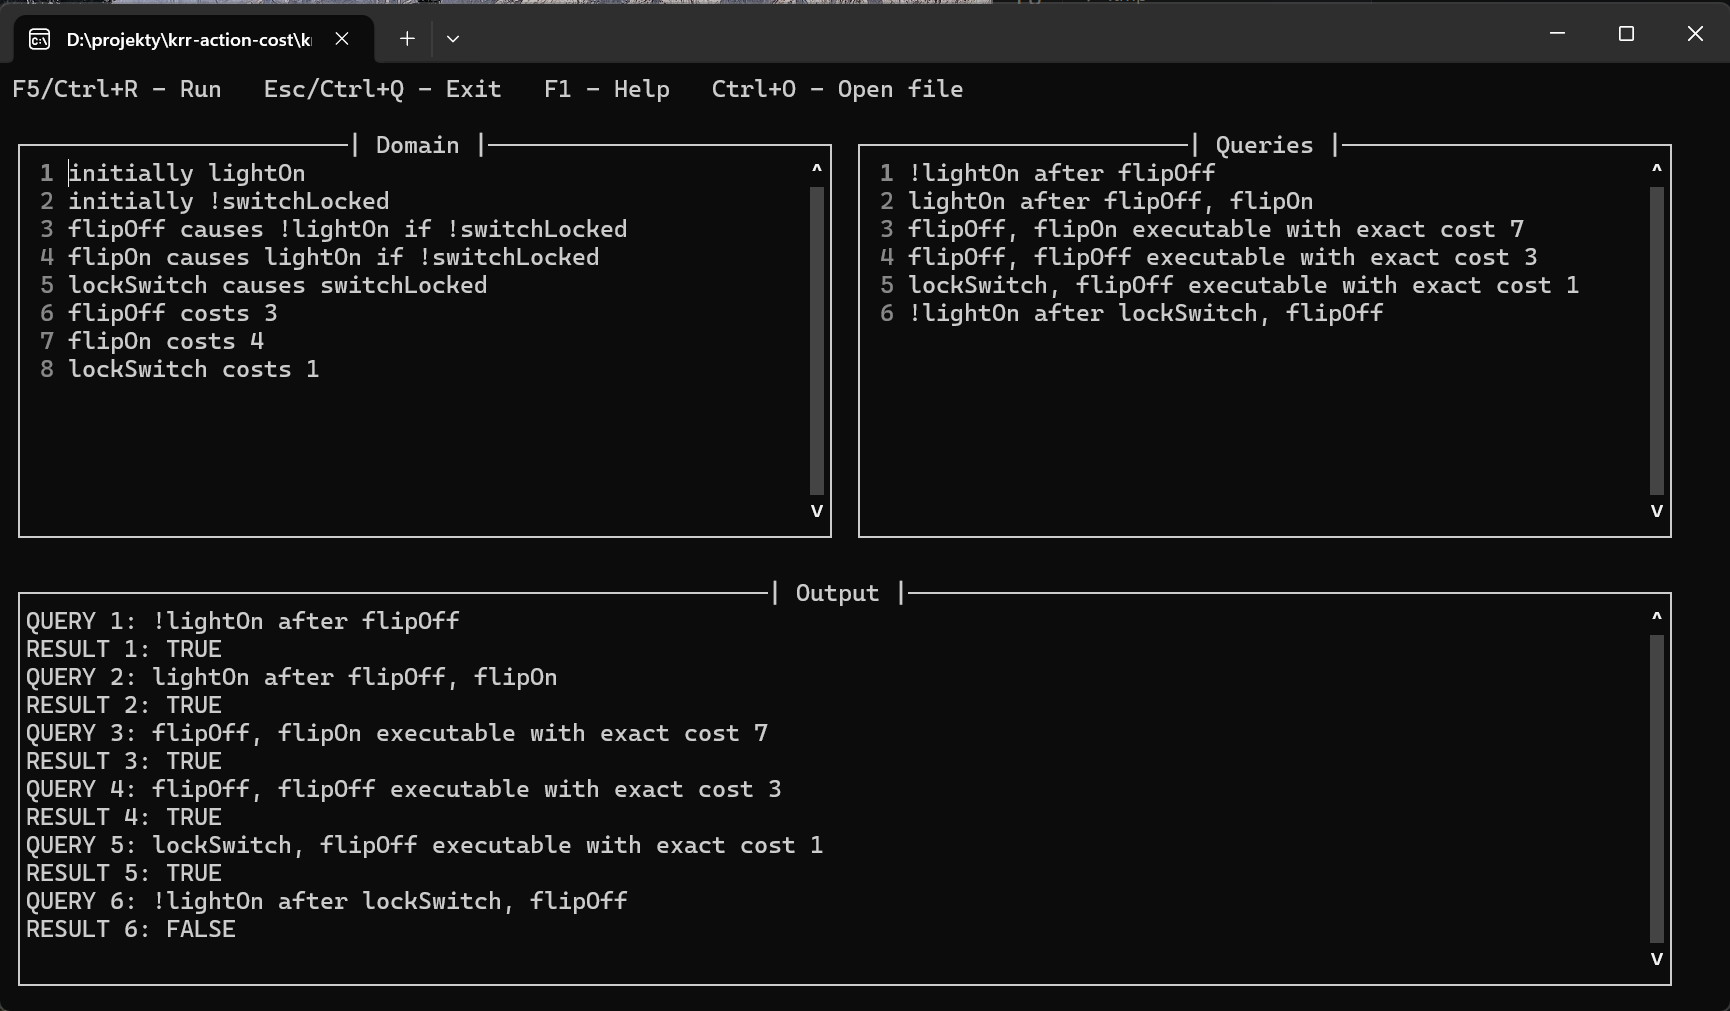
\includegraphics[width=0.8\textwidth]{testing/Kuba/example1.png}
    \caption{Jakub Seliga - example 1}
    \label{fig:JS1}
\end{figure}

\subsection*{Example 2: The Heater}
Let's consider a heater that warms a room, but only when the room is powered. The power status is unknown in the initial state, and there is no value statement to settle it, so both possibilities must be considered.
\subsubsection*{Action Domain Statements}
\[
\text{initially}~ \neg heated
\]
\[
warmUp ~\text{causes}~ heated ~\text{if}~ powered
\]
\[
warmUp ~\text{costs}~ 6
\]
\subsubsection*{Program}
\[
P = (warmUp)
\]
\subsubsection*{Complete initial states}
The fluent $powered$ is left unspecified, so two completions arise, and both are consistent since no value statement filters either out:
\[
\sigma_0^1 = \{\neg heated, powered\}
\]
\[
\sigma_0^2 = \{\neg heated, \neg powered\}
\]
\subsubsection*{Execution}
\paragraph{Case 1: $\sigma_0^1$}
Precondition holds, so:
\[
\sigma_1^1 = \{heated, powered\}
\]
Cost:
\[
Cost^\star(P) = 6
\]
\paragraph{Case 2: $\sigma_0^2$}
Precondition does not hold, so:
\[
\sigma_1^2 = \{\neg heated, \neg powered\}
\]
Cost:
\[
Cost^\star(P) = 0
\]
\subsubsection*{Final States}
\[
\{\sigma_1^1, \sigma_1^2\}
\]
\subsubsection*{Query Results}
\paragraph{Q1: Goal Satisfaction}
\[
\{heated\} ~\text{after}~ warmUp
\]
is false because $heated$ does not hold in all final states.
\[
\{heated\} ~\text{after}~ warmUp, warmUp
\]
is false for the same reason.
\paragraph{Q2 and Q3: Executability with Cost}
\[
P ~\text{executable with cost}~ 6
\]
is true since for all executions:
\[
Cost^\star(P) \leq 6
\]
\[
P ~\text{executable with exact cost}~ 6
\]
is false since $Cost^\star(P)$ is not always 6.
\[
warmUp, warmUp ~\text{executable with cost}~ 6
\]
is true, because the second $warmUp$ is idempotent in the powered branch, so the total cost remains 6.
\subsubsection*{Print screen}
\begin{figure}[H]
    \centering
    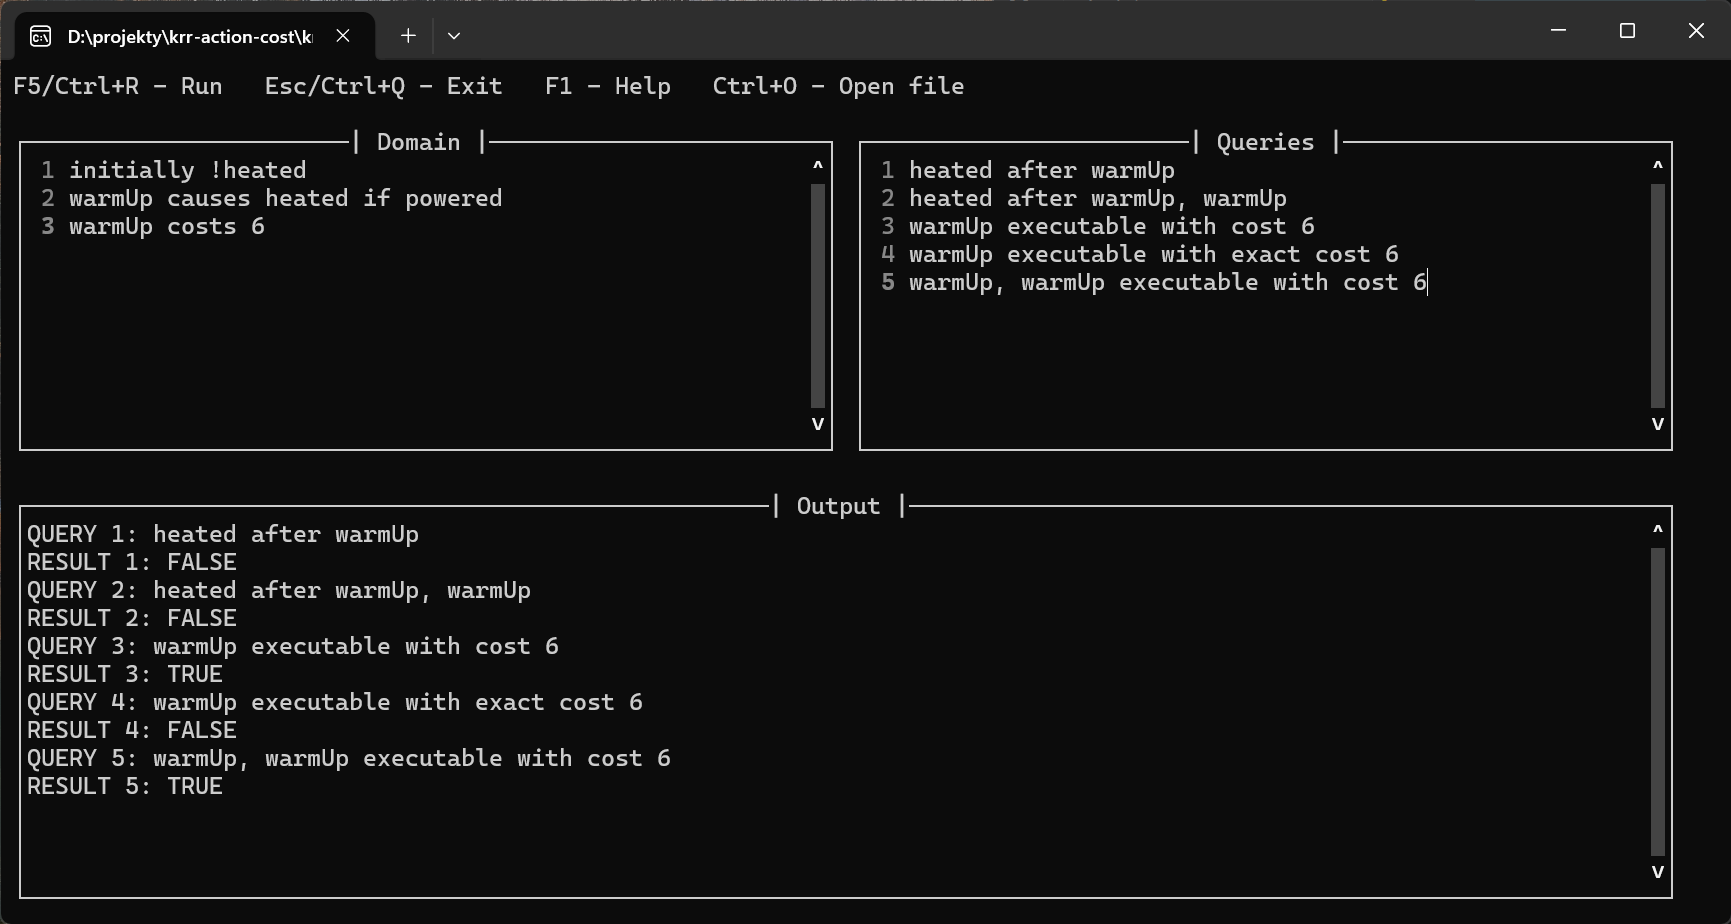
\includegraphics[width=0.8\textwidth]{testing/Kuba/example2.png}
    \caption{Jakub Seliga - example 2}
    \label{fig:JS2}
\end{figure}
\subsection*{Example 3: The Polishing Bench}
Let's consider a workpiece that can be polished or buffed. Polishing requires the piece to be clean, and a value statement enforces that polishing always yields a polished piece. The cleanliness of the piece is unspecified initially, but the value statements collapse this uncertainty to a single model.
\subsubsection*{Action Domain Statements}
\[
\text{initially}~ \neg polished
\]
\[
polished ~\text{after}~ polish
\]
\[
polish ~\text{causes}~ polished ~\text{if}~ clean
\]
\[
clean ~\text{after}~ polish
\]
\[
polish ~\text{costs}~ 4
\]
\[
buff ~\text{causes}~ polished
\]
\[
buff ~\text{costs}~ 2
\]
\subsubsection*{Complete initial states}
The fluent $clean$ is unspecified, giving two candidate completions:
\[
\sigma_0^1 = \{\neg polished, clean\}
\]
\[
\sigma_0^2 = \{\neg polished, \neg clean\}
\]
However, $\sigma_0^2$ is not consistent with the action domain.
Indeed, since $clean$ does not hold, the conditional effect of $polish$ does not apply, and by inertia:
\[
\Psi(polish, \sigma_0^2) \models \neg polished
\]
But the value statement requires:
\[
\Psi(polish, \sigma_0^2) \models polished
\]
This is a contradiction. Therefore, $\sigma_0^2$ is not allowed.

\subsubsection*{Execution}
Thus, the only possible initial state is:
\[
\sigma_0 = \{\neg polished, clean\}
\]
\paragraph{Action $polish$}
The precondition $clean$ holds, so $polished$ becomes true while $clean$ is untouched:
\[
\sigma_1 = \{polished, clean\}
\]
\[
Cost(polish, \sigma_0) = 4
\]
\paragraph{Repeated actions}
A second $polish$, or a following $buff$, finds $polished$ already true, so no change occurs and the empty effect rule gives cost 0.
\subsubsection*{Final States}
\[
\{\sigma_1\}
\]
\subsubsection*{Query Results}
\paragraph{Q1: Goal Satisfaction}
\[
\{polished\} ~\text{after}~ polish
\]
is true.
\[
\{clean\} ~\text{after}~ polish
\]
is true.
\[
\{polished\} ~\text{after}~ buff
\]
is true.
\paragraph{Q2: Executability with Cost}
\[
polish ~\text{executable with exact cost}~ 4
\]
is true.
\[
buff ~\text{executable with exact cost}~ 2
\]
is true.
\paragraph{Q3: Executability with exact Cost}
\[
polish, polish ~\text{executable with exact cost}~ 4
\]
is true, because the repeated $polish$ re-asserts an already-true fluent and adds zero cost.
\[
polish, buff ~\text{executable with exact cost}~ 4
\]
is true, since $buff$ produces an empty effect after the piece is polished.
\[
buff, buff ~\text{executable with exact cost}~ 2
\]
is true, for the same reason.
\subsubsection*{Print screen}
\begin{figure}[H]
    \centering
    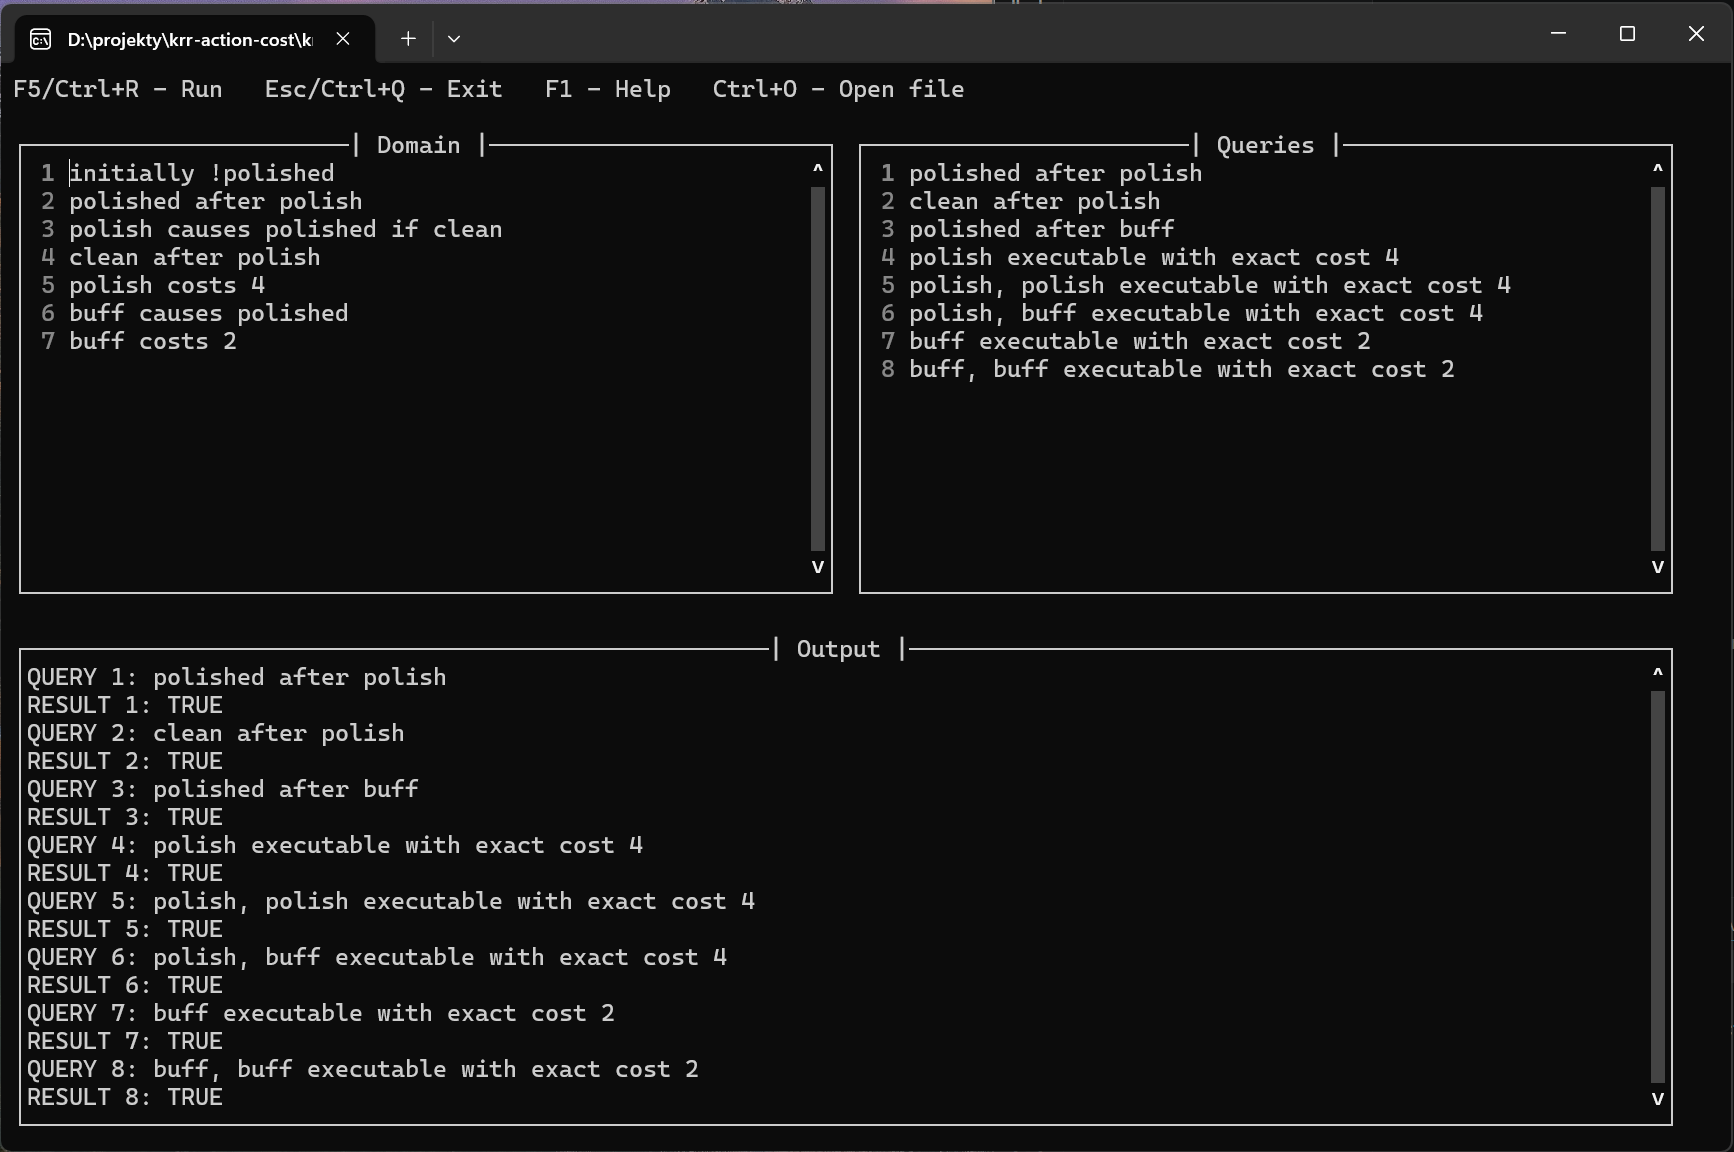
\includegraphics[width=0.8\textwidth]{testing/Kuba/example3.png}
    \caption{Jakub Seliga - example 3}
    \label{fig:JS3}
\end{figure}

\subsection*{Example 4: The Automated Bottling Line}
Consider an automated bottling line with three stages. In the first stage, an empty bottle is positioned by a gravity-fed chute. Because this operation does not require any powered mechanism, no cost statement is assigned to it. In the next two stages, the bottle is filled by an electric pump and sealed by a hydraulic press, both of which consume resources and therefore have associated costs. This scenario demonstrates the two cases in which the cost of an action is zero under assumption A5: when no cost statement is defined for the action, and when the action is defined with a cost but results in no state change.
\subsubsection*{Action Domain Statements}
\[
\text{initially}~ \neg bottleLoaded
\]
\[
\text{initially}~ \neg bottleFilled
\]
\[
\text{initially}~ \neg bottleCapped
\]
\[
loadBottle ~\text{causes}~ bottleLoaded
\]
\[
fillBottle ~\text{causes}~ bottleFilled ~\text{if}~ bottleLoaded
\]
\[
capBottle ~\text{causes}~ bottleCapped ~\text{if}~ bottleFilled
\]
\[
fillBottle ~\text{costs}~ 4
\]
\[
capBottle ~\text{costs}~ 3
\]
\[
bottleCapped ~\text{after}~ loadBottle, fillBottle, capBottle
\]
\subsubsection*{Program}
\[
P = (loadBottle, fillBottle, capBottle)
\]
\subsubsection*{Complete initial states}
All three fluents are fixed by the initial statements, so the initial state is complete and there is a single candidate model:
\[
\sigma_0 = \{\neg bottleLoaded, \neg bottleFilled, \neg bottleCapped\}
\]
This candidate must still satisfy the value statement $bottleCapped ~\text{after}~ loadBottle, fillBottle, capBottle$. Running the full program from $\sigma_0$ (traced below) ends in a state where $bottleCapped$ holds, so the checkpoint is satisfied and the model survives.
\subsubsection*{Execution}
\paragraph{Action 1: $loadBottle$}
The effect is unconditional, so $bottleLoaded$ turns true:
\[
\sigma_1 = \{bottleLoaded, \neg bottleFilled, \neg bottleCapped\}
\]
Cost calculation: although the state changed ($\Psi(loadBottle, \sigma_0) \neq \sigma_0$), the action $loadBottle$ has \emph{no} cost statement in the domain. By assumption A5 an action whose cost is unspecified contributes zero, so:
\[
Cost(loadBottle, \sigma_0) = 0
\]
\paragraph{Action 2: $fillBottle$}
The precondition $bottleLoaded$ holds, so the pump fills the bottle:
\[
\sigma_2 = \{bottleLoaded, bottleFilled, \neg bottleCapped\}
\]
Cost calculation: the state changed and $fillBottle$ has a declared cost, so:
\[
Cost(fillBottle, \sigma_1) = 4
\]
\paragraph{Action 3: $capBottle$}
The precondition $bottleFilled$ holds, so the press caps the bottle:
\[
\sigma_3 = \{bottleLoaded, bottleFilled, bottleCapped\}
\]
Cost calculation: the state changed and $capBottle$ has a declared cost, so:
\[
Cost(capBottle, \sigma_2) = 3
\]
\paragraph{Total Program Cost}
\[
Cost^\star(P) = 0 + 4 + 3 = 7
\]
\subsubsection*{Final States}
\[
\{\sigma_3\}
\]
\subsubsection*{Query Results}
\paragraph{Q1: Goal Satisfaction}
\[
\{bottleLoaded, bottleFilled, bottleCapped\} ~\text{after}~ loadBottle, fillBottle, capBottle
\]
is true because all three literals hold in the single final state $\sigma_3$.
\paragraph{Q2 and Q3: Executability with Cost}
\[
loadBottle ~\text{executable with exact cost}~ 0
\]
is true. The action changes the state, yet because no cost statement is declared for $loadBottle$ its cost is zero. This is the \emph{cost-unspecified} branch of the rule.
\[
fillBottle ~\text{executable with exact cost}~ 0
\]
is true, but for the opposite reason. Run alone from $\sigma_0$, the precondition $bottleLoaded$ of $fillBottle$ does not hold, so the action produces an empty effect; an empty effect costs zero even though $fillBottle$ has a declared cost of 4. This is the \emph{empty-effect} branch of the rule.
\[
loadBottle, fillBottle ~\text{executable with exact cost}~ 4
\]
is true, since the free $loadBottle$ first enables the precondition and contributes 0, after which $fillBottle$ changes the state and contributes 4.
\[
loadBottle, fillBottle, capBottle ~\text{executable with exact cost}~ 7
\]
is true since $Cost^\star(P) = 0 + 4 + 3 = 7$.
\[
loadBottle, fillBottle, capBottle ~\text{executable with cost}~ 7
\]
is true since for all executions $Cost^\star(P) \leq 7$.
\[
loadBottle, fillBottle, capBottle ~\text{executable with cost}~ 6
\]
is false since there exists an execution with cost $7 > 6$.

\subsubsection*{Print screen}
\begin{figure}[H]
    \centering
    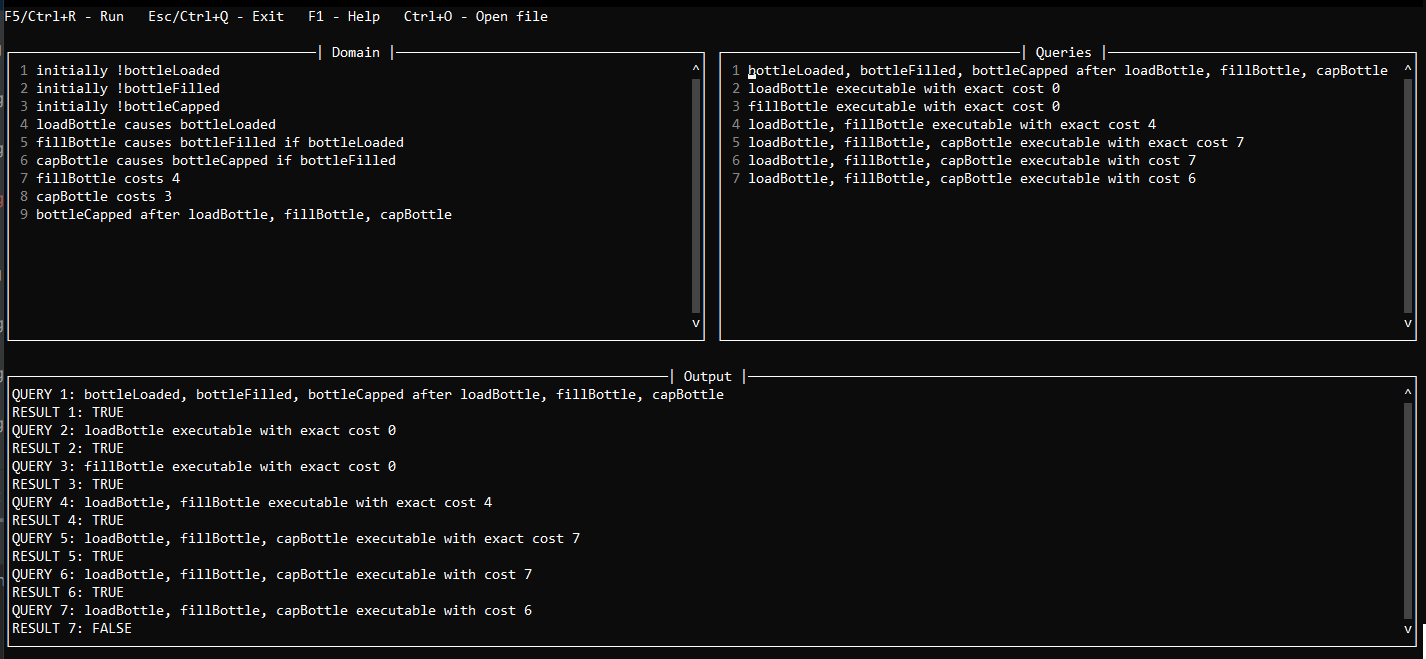
\includegraphics[width=0.8\textwidth]{testing/Kuba/example4.png}
    \caption{Jakub Seliga - example 4}
    \label{fig:JS4}
\end{figure}


\subsection*{Wiktoria Koniecko}
\subsection*{Example 1: YSP modification}
Let's consider a modification of the Yale Shooting Problem in which we don't care whether the gun is
loaded or not and two shots are necessary to kill the turkey.

\subsubsection*{Action Domain Statements}
\[\text{initially}~ alive\]
\[wounded ~\text{after}~ shoot\]
\[shoot ~\text{causes}~ \neg alive ~\text{if}~ wounded\]
\[shoot ~\text{causes}~ wounded ~\text{if}~ \neg wounded\]
\[shoot ~\text{costs}~ 5\]

\subsubsection*{Complete initial states}
The fluent $wounded$ is unspecified, giving two candidate completions:
\[\sigma_0^1 = \{alive, wounded\}\]
\[\sigma_0^2 = \{alive, \neg wounded\}\]

\subsubsection*{Execution}
The only available action is \(shoot\). If \(wounded\), performing \(shoot\) only once is sufficient
to kill the turkey and shooting will no longer have any effect, so any non-empty program will have
exact cost 5. If not \(wounded\), shooting two times is necessary, and the program will have cost
at most 10.

\subsubsection*{Print screen}
\begin{figure}[H]
    \centering
    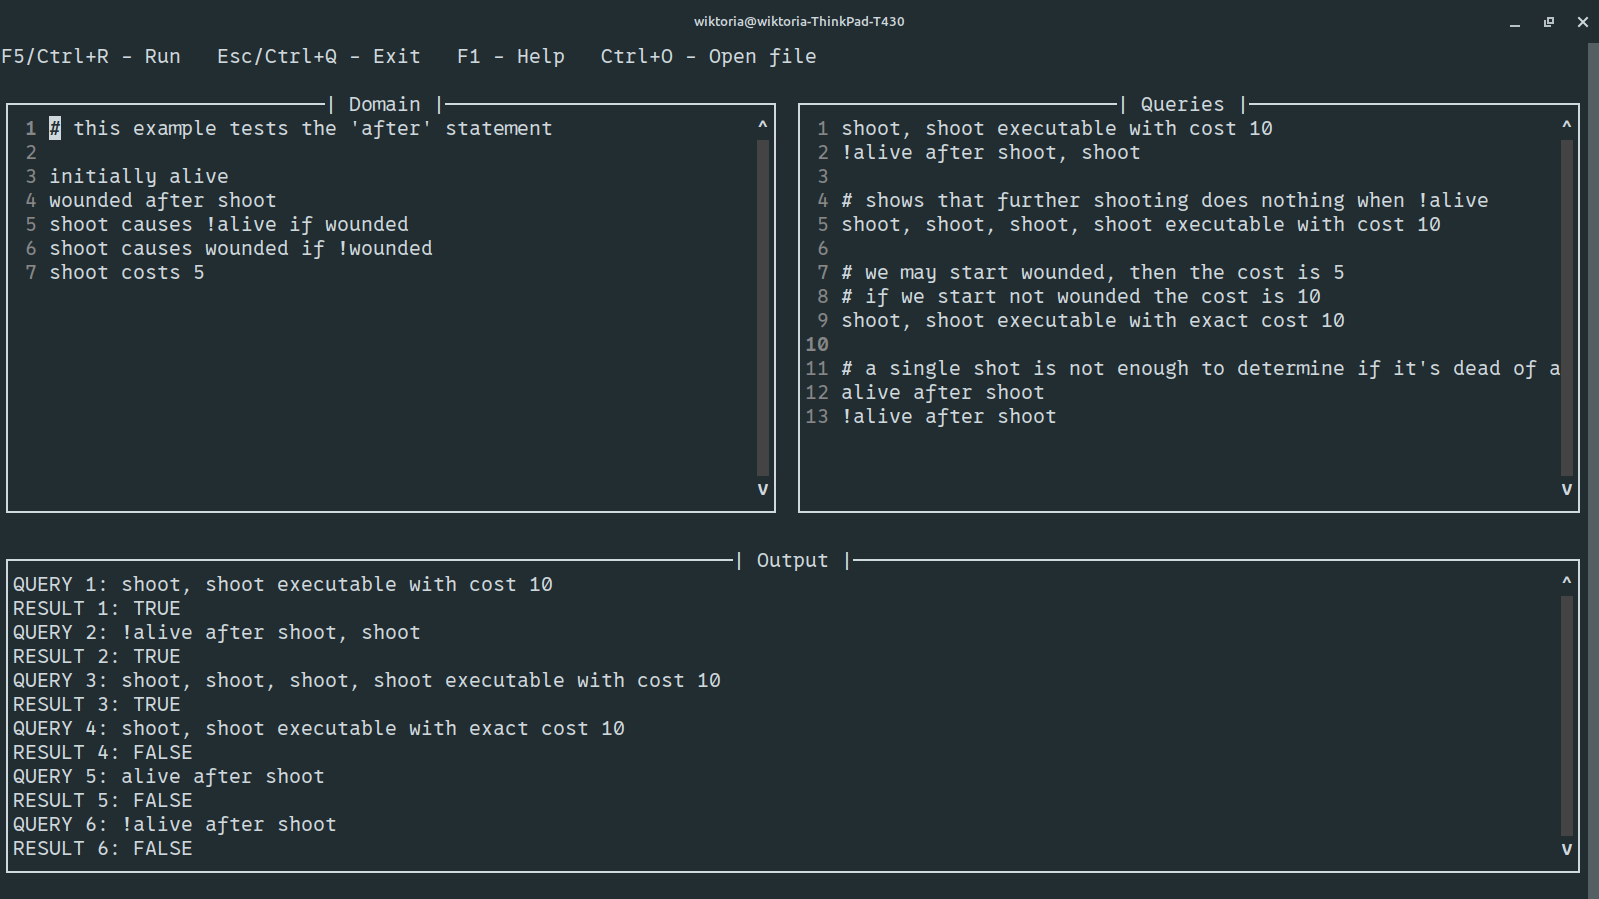
\includegraphics[width=0.8\textwidth]{testing/Wiktoria/example1.png}
    \caption{Wiktoria Koniecko - example 1}
    \label{fig:WK1}
\end{figure}

\subsubsection*{Query Results}
\paragraph{Q1: Goal Satisfaction}
\[\neg alive ~\text{after}~ shoot, shoot\]
is true. If the turkey was wounded, it dies with the first shot. If it wasn't, it dies with the second.

\[alive ~\text{after}~ shoot\]
\[\neg alive ~\text{after}~ shoot\]
are both false. We cannot tell whether the turkey is dead or alive after only being shot once.

\paragraph{Q2: Executability with cost}
\[shoot, shoot ~\text{executable with cost}~ 10\]
is true because the cost of \(shoot\) is 5.

\[shoot, shoot, shoot, shoot ~\text{executable with cost}~ 10\]
is true because after shooting twice the turkey is guaranteed to be dead, so the \(shoot\) action
has no effect and is performed with cost 0.

\paragraph{Q3: Executability with exact cost}
\[shoot, shoot ~\text{executable with exact cost}~ 10\]
is false. If the turkey is wounded it will die after the first shot. The second action would have
no effect, so the program would execute with cost 5.

\subsection*{Example 2: YSP modification 2: inconsistent domain}
This is an example of the Yale Shooting Problem modified to have an inconsistent domain.

\subsubsection*{Action Domain Statements}
\[\text{initially}~ alive, loaded\]
\[loaded ~\text{after}~ shoot\]
\[shoot ~\text{causes}~ \neg loaded, \neg alive ~\text{if}~ loaded\]
\[load ~\text{causes}~ loaded\]
\[shoot ~\text{costs}~ 5\]
\[load ~\text{costs}~ 2\]

\(loaded\) is undefined, because it has to be simultaneously true and false after performing shoot
in the initial state.

\subsubsection*{Print screen}
\begin{figure}[H]
    \centering
    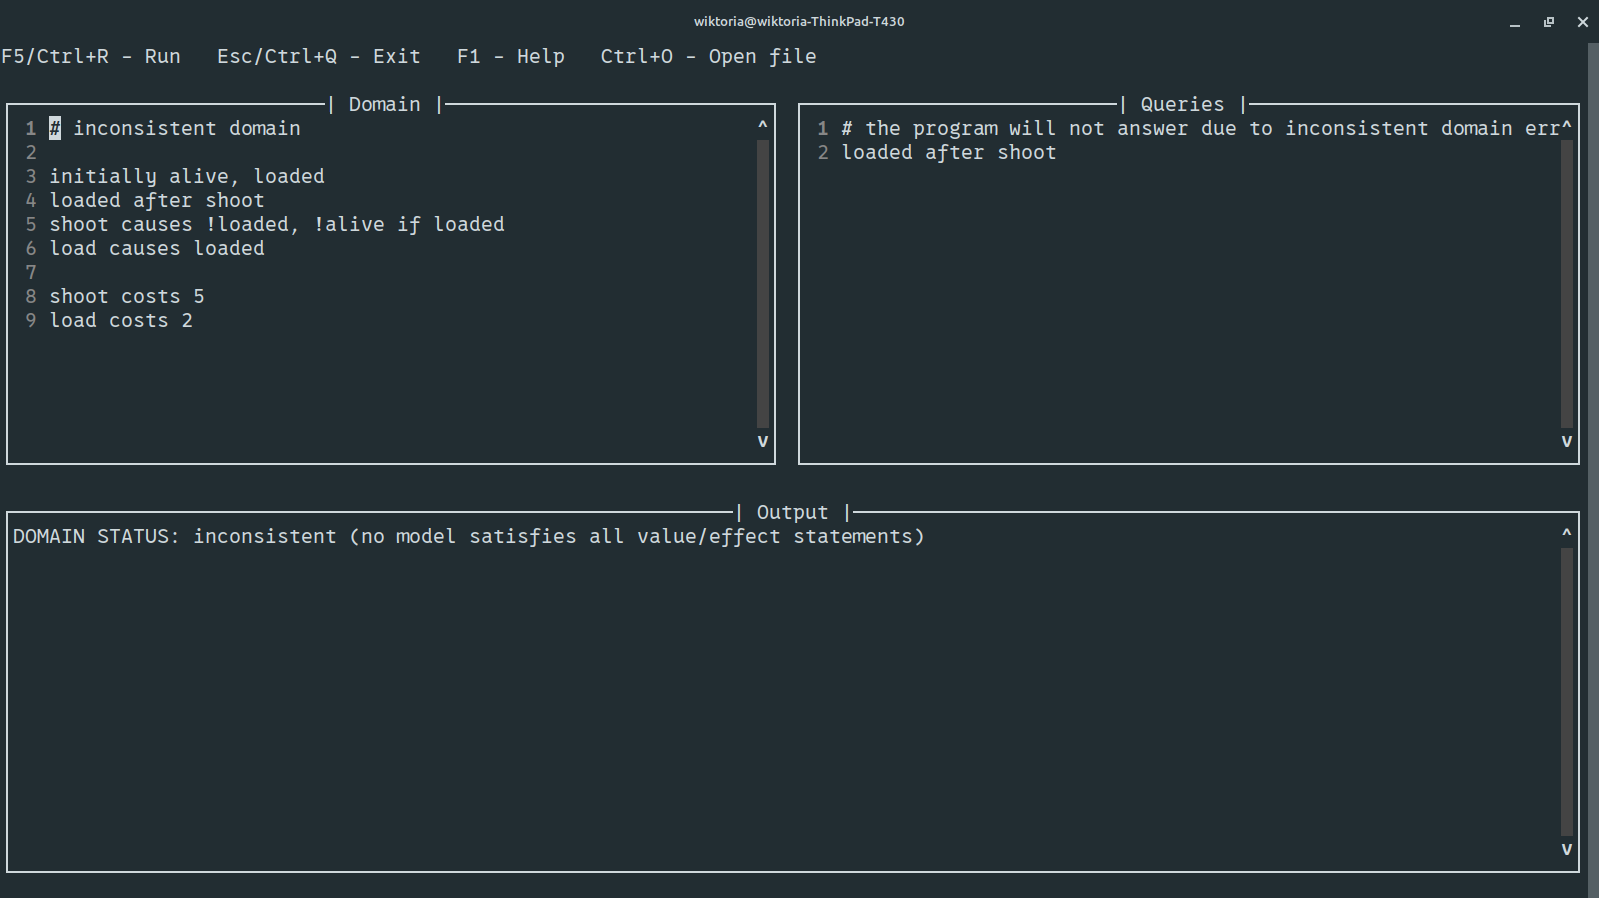
\includegraphics[width=0.8\textwidth]{testing/Wiktoria/example2.png}
    \caption{Wiktoria Koniecko - example 2}
    \label{fig:WK2}
\end{figure}

\subsection*{Example 3: Watering a plant}
This example models watering a plant. The plant dies if it doesn't receive water or is watered too much.

\subsubsection*{Action Domain Statements}
\[\text{initially}~ plantAlive\]
\[waterPlant ~\text{causes} plantWatered\]
\[waterPlant ~\text{causes} !plantAlive ~\text{if} plantWatered\]
\[wait ~\text{causes} !plantWatered\]
\[wait ~\text{causes} !plantAlive ~\text{if} !plantWatered\]
\[waterPlant ~\text{costs}~ 1\]
\[wait ~\text{costs} 9\]

\subsubsection*{Completions of $\sigma_0$}
\(plantWatered\) is unspecified. This gives us two completions:
\[\sigma_0^1 = \{plantAlive, plantWatered\}\]
\[\sigma_0^2 = \{plantAlive, \neg plantWatered\}\]

\subsubsection*{Execution}
The plant will surely not be alive if the program contains the same action twice in a row regardless of its
initial state. However, the death of the plant doesn't necessarily reduce the cost of all future actions to 0. Both actions
can still impact the fluent \(plantWatered\). Let's consider the following program:
\[waterPlant, wait, waterPlant, wait.\]
Regardless of whether the plant is alive or not, all the statements except the first change
\(plantWatered\), so they're executed with non-zero cost. The first statement changes \(plantWatered\)
if the plant was not initially watered. If it was, the plant becomes no longer alive, changing \(plantAlive\).
Thus the first statement is also executed with non-zero cost regardless of the initial state.

\subsubsection*{Query Results}
\paragraph{Q1: Goal Satisfaction}
\[\neg plantAlive ~\text{after}~ wait, wait\]
\[\neg plantAlive ~\text{after}~ waterPlant, waterPlant\]
are both true.

\[alive ~\text{after}~ waterPlant, wait, waterPlant, wait\]
\[\neg alive ~\text{after}~ waterPlant, wait, waterPlant, wait\]
are both false. We cannot tell whether the plant is dead or alive.

\paragraph{Q2: Executability with cost}
\[wait, wait ~\text{executable with cost}~ 18\]
is true because the \(wait\) action will have an effect at most twice and its cost is 9.

\paragraph{Q3: Executability with exact cost}
\[waterPlant, wait, waterPlant, wait ~\text{executable with exact cost}~ 20\]
is true.

\[waterPlant, waterPlant, waterPlant, waterPlant ~\text{executable with exact cost}~ 2\]
is false. If the plant was initially watered, the program would execute with cost 1.

\subsubsection*{Print screen}
\begin{figure}[H]
    \centering
    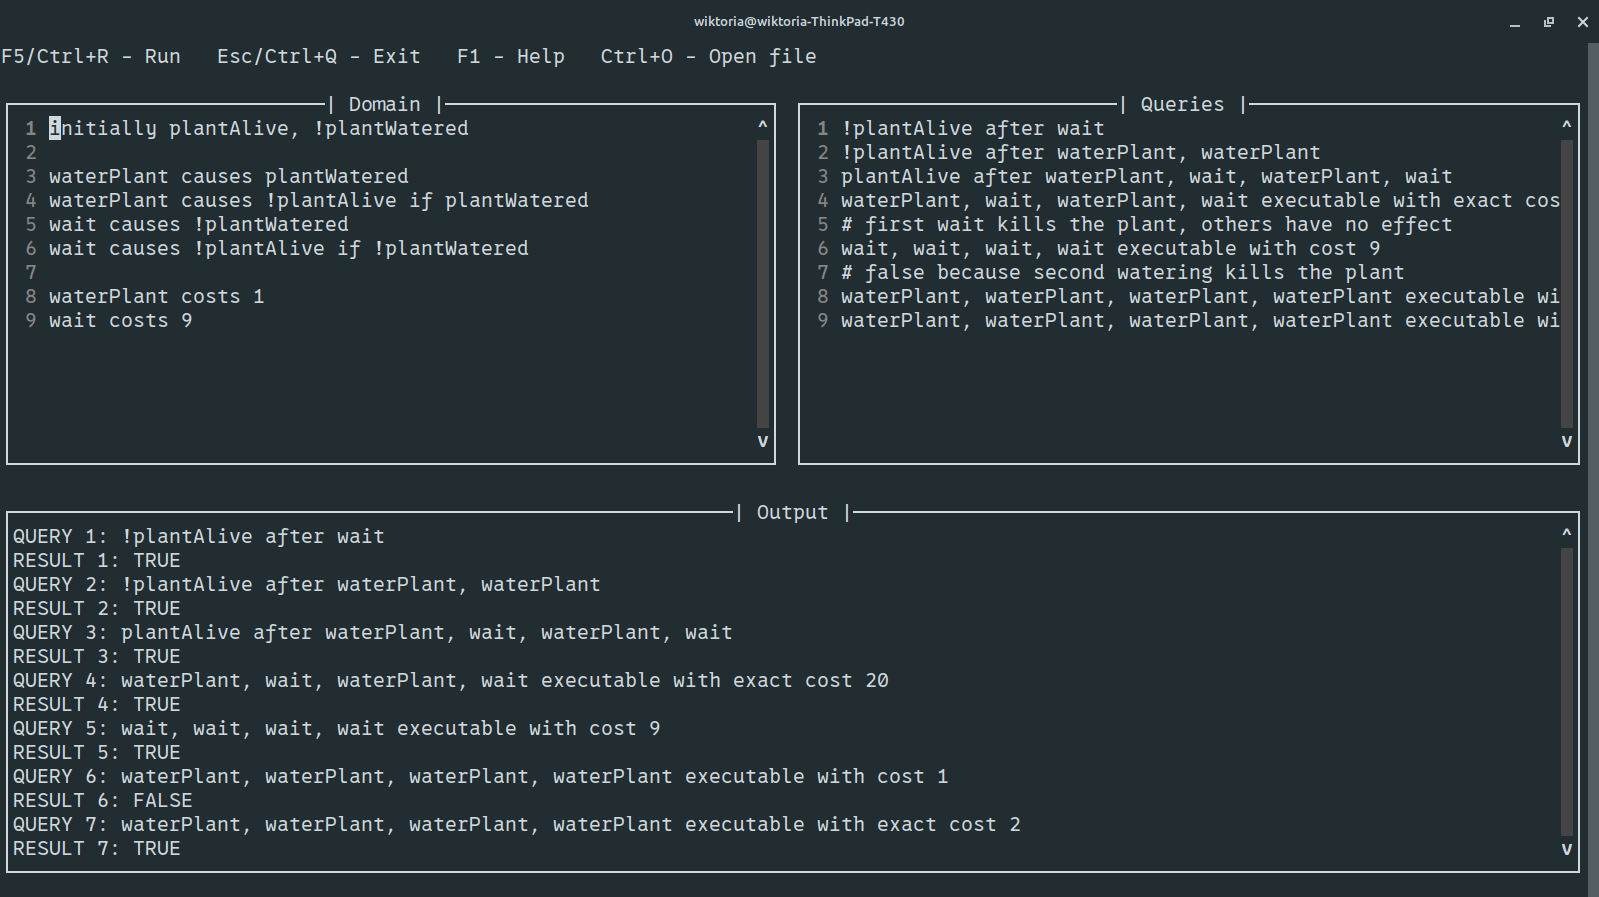
\includegraphics[width=0.8\textwidth]{testing/Wiktoria/example3.png}
    \caption{Wiktoria Koniecko - example 3}
    \label{fig:WK3}
\end{figure}

\subsection*{Sebastian Trojan}

\subsection*{Example 1: The Inspection Drone}
The drone is initially not ready and not airborne. Inspecting the drone makes
it ready. Launching the drone makes it airborne if it is ready, and launching
costs 6. The program inspects the drone twice and then launches it twice.

\subsubsection*{Action Domain Statements}
\[
\text{initially}~ \neg droneReady
\]
\[
\text{initially}~ \neg airborne
\]
\[
inspectDrone ~\text{causes}~ droneReady
\]
\[
launchDrone ~\text{causes}~ airborne ~\text{if}~ droneReady
\]
\[
launchDrone ~\text{costs}~ 6
\]

\subsubsection*{Program}
\[
P = (inspectDrone, inspectDrone, launchDrone, launchDrone)
\]

\subsubsection*{How it works}
The first inspection changes the state, but because no cost statement is
declared for \(inspectDrone\), it still costs \(0\). The second inspection is
both cost-unspecified and an empty effect, so it also costs \(0\). The first
launch changes the fluent \(airborne\) and therefore costs \(6\), while the
second launch has no further effect and costs \(0\).

\subsubsection*{Queries}
\[
\{airborne\} ~\text{after}~ P
\]
is true.
\[
P ~\text{executable with exact cost}~ 6
\]
is true.
\[
inspectDrone ~\text{executable with exact cost}~ 0
\]
is true.

\subsubsection*{Print screen}
\begin{figure}[H]
    \centering
    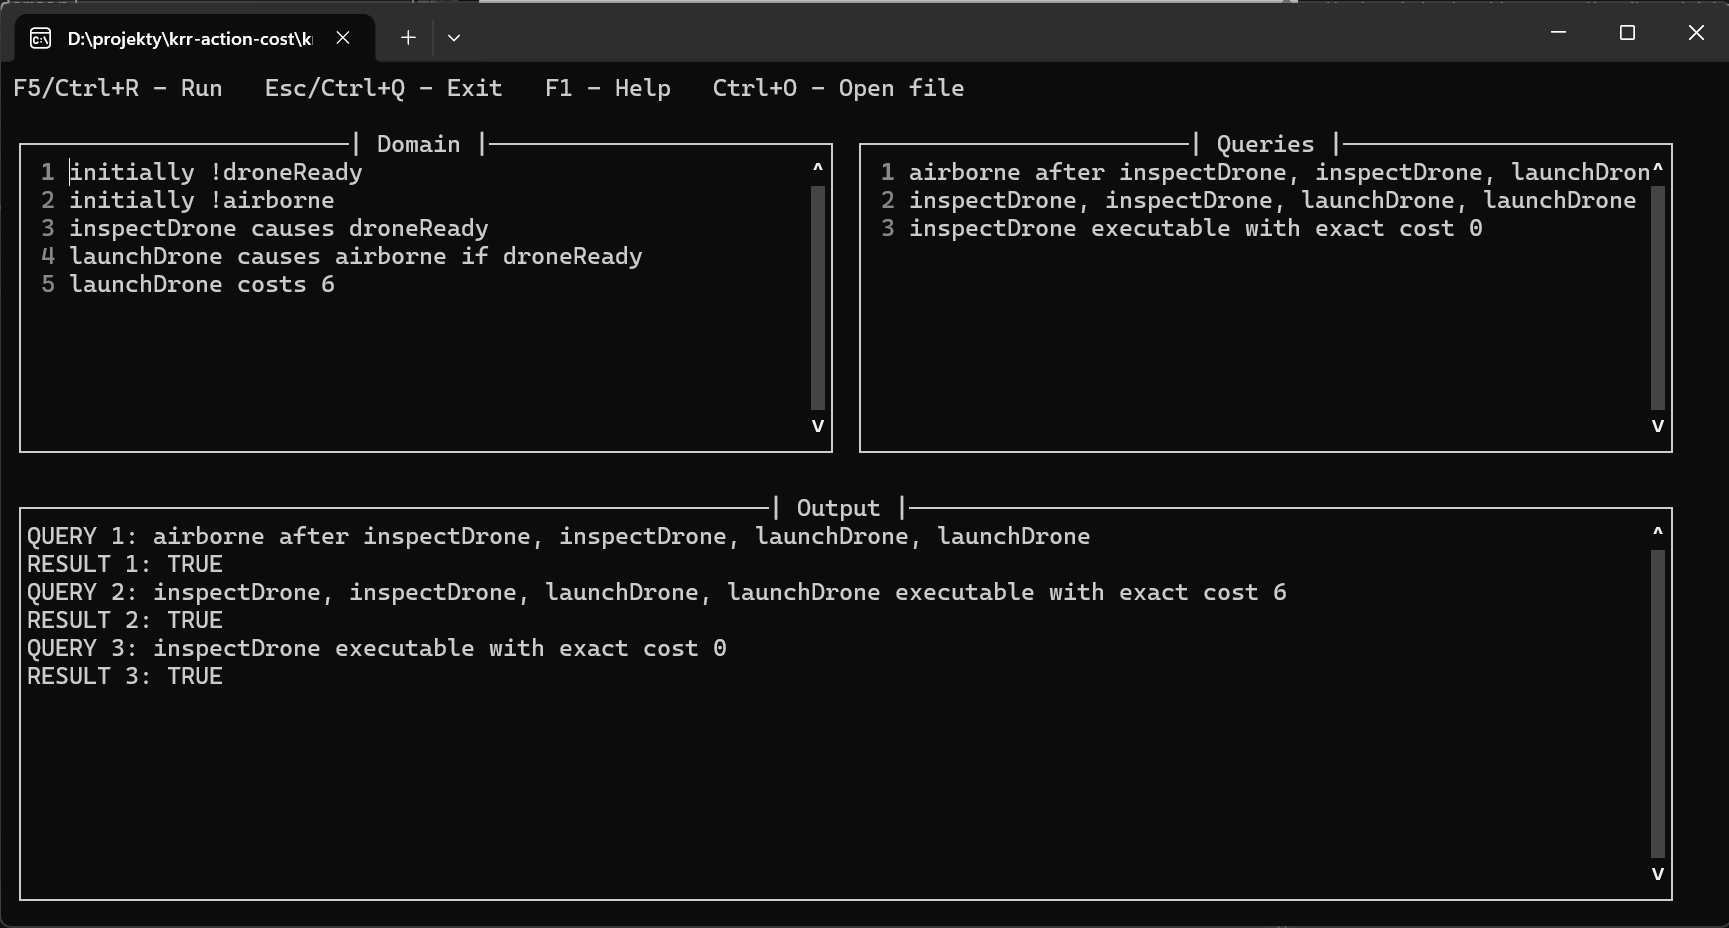
\includegraphics[width=0.8\textwidth]{testing/Sebastian/example1.png}
    \caption{Sebastian Trojan - example 1}
    \label{fig:ST1}
\end{figure}

\subsection*{Example 2: The Security Gate}
The gate is initially closed. It is not known whether the employee badge is
valid. Scanning the badge opens the gate if the badge is valid, and scanning
costs 3. The program scans the badge once.

\subsubsection*{Action Domain Statements}
\[
\text{initially}~ \neg gateOpen
\]
\[
\text{scanBadge} ~\text{causes}~ gateOpen ~\text{if}~ badgeValid
\]
\[
\text{scanBadge} ~\text{costs}~ 3
\]

\subsubsection*{Program}
\[
P = (scanBadge)
\]

\subsubsection*{How it works}
Because the fluent \(badgeValid\) is not fixed initially, there are two
models. In one model the badge is valid, so scanning it opens the gate and the
cost is \(3\). In the second model the badge is not valid, so the action has
an empty effect and costs \(0\). This gives two different final states and two
different total costs for the same program.

\subsubsection*{Queries}
\[
\{gateOpen\} ~\text{after}~ P
\]
is false.
\[
P ~\text{executable with cost}~ 3
\]
is true.
\[
P ~\text{executable with exact cost}~ 3
\]
is false.

\subsubsection*{Print screen}
\begin{figure}[H]
    \centering
    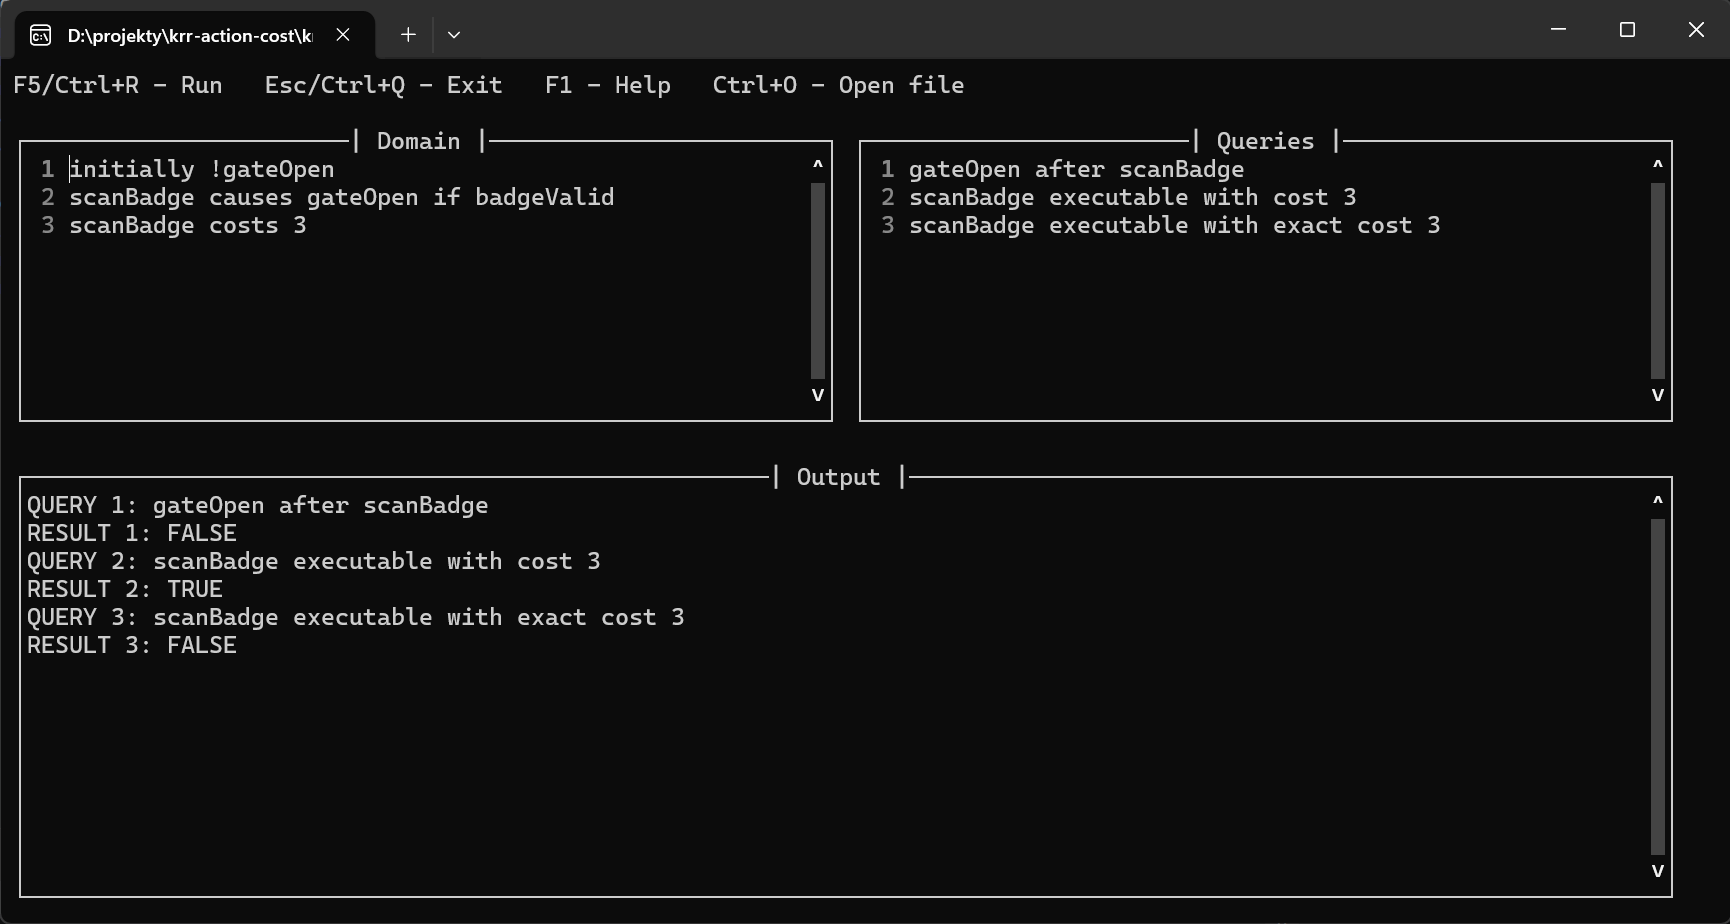
\includegraphics[width=0.8\textwidth]{testing/Sebastian/example2.png}
    \caption{Sebastian Trojan - example 2}
    \label{fig:ST2}
\end{figure}

\subsection*{Example 3: The Cooling Console}
Cooling is initially off. It is not known whether the filter is blocked.
Cleaning the filter makes it not blocked and costs 2. Starting cooling makes
cooling active if the filter is not blocked, and starting costs 4. The value
statement requires cooling to be on after first trying to start cooling and
then cleaning the filter.

\subsubsection*{Action Domain Statements}
\[
\text{initially}~ \neg coolingOn
\]
\[
coolingOn ~\text{after}~ startCooling, cleanFilter
\]
\[
cleanFilter ~\text{causes}~ \neg filterBlocked
\]
\[
startCooling ~\text{causes}~ coolingOn ~\text{if}~ \neg filterBlocked
\]
\[
cleanFilter ~\text{costs}~ 2
\]
\[
startCooling ~\text{costs}~ 4
\]

\subsubsection*{Program}
\[
P = (startCooling, cleanFilter)
\]

\subsubsection*{How it works}
The fluent \(filterBlocked\) is initially unspecified, so there are two
candidate complete initial states. If the filter is already clear, then
\(startCooling\) succeeds and the value statement is satisfied. If the filter
is blocked, then \(startCooling\) has an empty effect and \(cleanFilter\) works
too late to make \(coolingOn\) true at the end of the program. That second
candidate is therefore filtered out, leaving only one valid model.

\subsubsection*{Queries}
\[
\{coolingOn\} ~\text{after}~ P
\]
is true.
\[
P ~\text{executable with cost}~ 4
\]
is true.
\[
P ~\text{executable with exact cost}~ 4
\]
is true.

\subsubsection*{Print screen}
\begin{figure}[H]
    \centering
    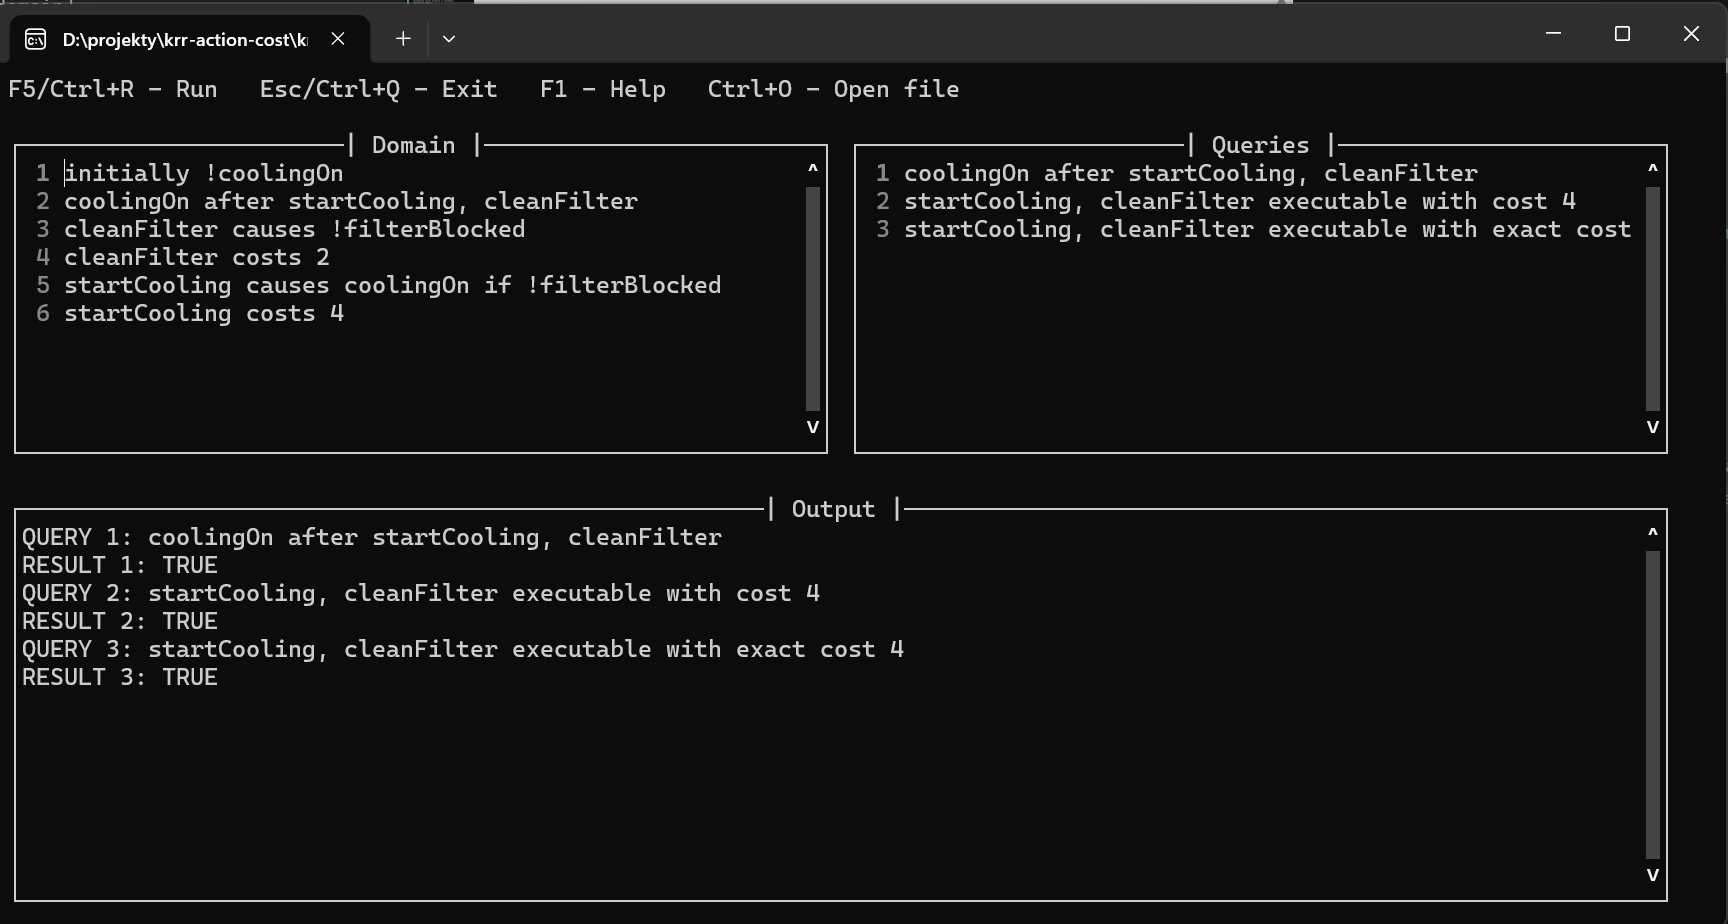
\includegraphics[width=0.8\textwidth]{testing/Sebastian/example3.png}
    \caption{Sebastian Trojan - example 3}
    \label{fig:ST3}
\end{figure}

\subsection*{Example 4: The Rocket Platform}
The rocket is initially not launched and its clamps are locked. Releasing the
clamps makes them unlocked and costs 3. Igniting launches the rocket only if
the clamps are already unlocked, and ignition costs 9. The value statement
requires the rocket to be launched after first igniting and then releasing the
clamps.

\subsubsection*{Action Domain Statements}
\[
\text{initially}~ \neg launched
\]
\[
\text{initially}~ clampsLocked
\]
\[
launched ~\text{after}~ ignite, releaseClamps
\]
\[
releaseClamps ~\text{causes}~ \neg clampsLocked
\]
\[
ignite ~\text{causes}~ launched ~\text{if}~ \neg clampsLocked
\]
\[
releaseClamps ~\text{costs}~ 3
\]
\[
ignite ~\text{costs}~ 9
\]

\subsubsection*{Program}
\[
P = (ignite, releaseClamps)
\]

\subsubsection*{How it works}
The initial state is fully specified, so there is only one candidate model.
However, \(ignite\) is executed while the clamps are still locked, so it cannot
cause \(launched\). The later action \(releaseClamps\) changes the state, but it
comes too late to rescue the failed launch. Since the value statement requires
\(launched\) after the whole program, no model can satisfy the domain.

\subsubsection*{Print screen}
\begin{figure}[H]
    \centering
    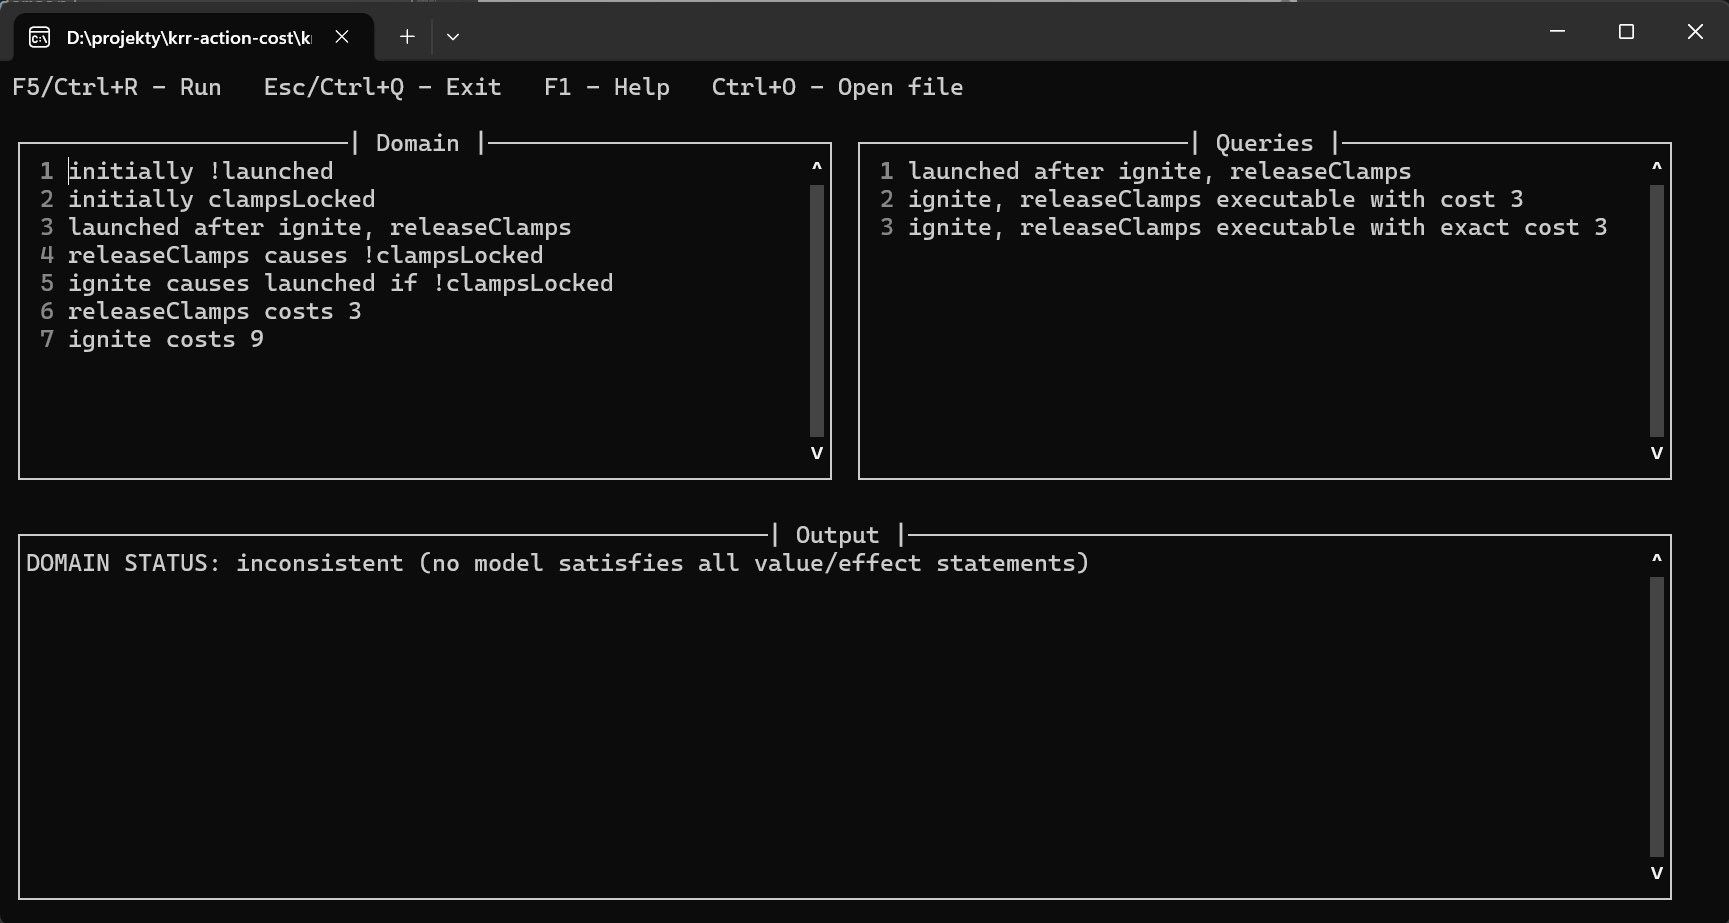
\includegraphics[width=0.8\textwidth]{testing/Sebastian/example4.png}
    \caption{Sebastian Trojan - example 4}
    \label{fig:ST4}
\end{figure}

\section{User guide}
The compiler is intended to be used through the prepared Windows executable.
After launching the application, the user may either enter a specification
directly in the editor or open an existing \texttt{.krr} or \texttt{.txt} file.
The left pane is used for domain statements, the right pane for queries, and the
output pane displays the compilation result.

\subsection{Specification format}
A stored specification should contain two sections:
\begin{verbatim}
[domain]
... domain statements ...

[queries]
... query statements ...
\end{verbatim}

The domain section may contain:
\begin{itemize}
    \item \texttt{initially fluent} or \texttt{initially !fluent}
    \item \texttt{fluent after action\_1, action\_2, ...}
    \item \texttt{action causes fluent if fluent, !fluent, ...}
    \item \texttt{action causes fluent}
    \item \texttt{action costs n}
\end{itemize}

The queries section may contain:
\begin{itemize}
    \item goal queries of the form
    \texttt{fluent, !fluent after action\_1, action\_2, ...}
    \item bounded-cost queries of the form
    \texttt{action\_1, action\_2 executable with cost n}
    \item exact-cost queries of the form
    \texttt{action\_1, action\_2 executable with exact cost n}
\end{itemize}

Negation is written only with the symbol \texttt{!}. Comments begin with
\texttt{\#}. Files may use either the \texttt{.krr} or \texttt{.txt} extension.

\subsection{Using the application}
The normal workflow is:
\begin{itemize}
    \item launch the executable,
    \item type the domain in the left pane and the queries in the right pane,
    or open an existing specification file with \texttt{Ctrl+O},
    \item press \texttt{F5} or \texttt{Ctrl+R} to run the compiler,
    \item read the result in the output pane.
\end{itemize}

The most important shortcuts are:
\begin{itemize}
    \item \texttt{F5} or \texttt{Ctrl+R} -- run the compiler,
    \item \texttt{Esc} or \texttt{Ctrl+Q} -- close the editor,
    \item \texttt{F1} -- show or hide help,
    \item \texttt{Ctrl+O} -- open an existing \texttt{.krr} or \texttt{.txt} file,
    \item \texttt{Tab} and \texttt{Shift+Tab} -- switch between panes.
\end{itemize}

The domain may remain unchanged while the user edits the query pane and reruns
the compiler multiple times. This makes the application convenient for testing
many queries against the same action domain.

\subsection{Output interpretation}
For a consistent domain, the compiler prints every query together with the
corresponding result \texttt{TRUE} or \texttt{FALSE}. If the domain is
inconsistent, the compiler prints only:
\begin{verbatim}
The domain is inconsistent.
\end{verbatim}
and query evaluation is skipped.


\section{Contribution}
For the parts of the report assessed jointly, all team members contributed equally.
The scope of testing performed by individual team members is described in the
``Testing'' section, so it is not included in the list below. Most of the report
and code were developed collaboratively, while the following list presents the
main area of responsibility assigned to each person in the project.

\begin{itemize}
    \item \textbf{Jakub Seliga -- 25\%}: implementation of the parser for the
    action language and query language, including the processing of domain and
    query statements from the specification format, as well as preparation of the
    example part of the report, including the construction and description of
    example domains and illustrative scenarios.
    \item \textbf{Michal Szewczak -- 25\%}: implementation of the graphical user
    interface and executable application, including file handling and user
    interaction, as well as preparation of the introduction, technical description
    of the adopted data structures and algorithms, and the user guide.
    \item \textbf{Sebastian Trojan -- 25\%}: implementation of the core compiler,
    including the construction of states, transition and cost tables, model
    generation, and query evaluation.
    \item \textbf{Wiktoria Koniecko -- 25\%}: preparation and refinement of the
    formal theoretical part of the report, especially the syntax and semantics of
    the action language and query language, as well as notation consistency.
\end{itemize}
\end{document}
